% Build: latexmk -pdf -interaction=nonstopmode -halt-on-error locus.tex
% Self-contained source; all diagrams are drawn with TikZ.
\documentclass[11pt,letterpaper]{article}
\usepackage[T1]{fontenc}
\usepackage[utf8]{inputenc}
\usepackage{lmodern,microtype}
\usepackage[margin=1in,headheight=15pt]{geometry}
\usepackage{amsmath,amssymb,amsthm,mathtools}
\usepackage{booktabs,tabularx,longtable,array}
\usepackage{enumitem,xcolor,listings,tikz,needspace,fancyhdr,titlesec}
\usepackage{etoolbox,xurl}
\usetikzlibrary{arrows.meta,positioning,fit}
\usepackage[colorlinks=true,linkcolor=ink,citecolor=accent,urlcolor=accent]{hyperref}
\usepackage{bookmark}
\definecolor{ink}{HTML}{22384A}
\definecolor{accent}{HTML}{28756E}
\definecolor{paperpanel}{HTML}{F2F5F3}
\definecolor{rulegray}{HTML}{CAD4D0}
\titleformat{\section}{\Large\sffamily\bfseries\color{ink}}{\thesection}{.65em}{}
\titleformat{\subsection}{\large\sffamily\bfseries\color{ink}}{\thesubsection}{.6em}{}
\titleformat{\subsubsection}{\normalsize\sffamily\bfseries}{\thesubsubsection}{.6em}{}
\pretocmd{\section}{\Needspace{6\baselineskip}}{}{}
\pretocmd{\subsection}{\Needspace{4\baselineskip}}{}{}
\setlength{\parindent}{0pt}
\setlength{\parskip}{.43em}
\setlength{\emergencystretch}{2.5em}
\setcounter{tocdepth}{1}
\setlist{nosep,leftmargin=1.6em}
\renewcommand{\arraystretch}{1.15}
\newcolumntype{Y}{>{\raggedright\arraybackslash}X}
\newcolumntype{P}[1]{>{\raggedright\arraybackslash}p{#1}}
\newcommand{\code}[1]{\nolinkurl{#1}}
\newcommand{\N}{\mathbb N}
\newcommand{\Z}{\mathbb Z}
\newcommand{\Q}{\mathbb Q}
\newcommand{\R}{\mathbb R}
\newcommand{\C}{\mathbb C}
\newcommand{\Spec}{\operatorname{Spec}}
\newcommand{\den}[1]{[\![#1]\!]}
\newcommand{\jet}[2]{\operatorname{Jet}_{#1}(#2)}
\newcommand{\ord}{\operatorname{ord}}
\newcommand{\Locus}{\textsc{Locus}}
\newtheorem{theorem}{Theorem}[section]
\newtheorem{proposition}[theorem]{Proposition}
\newtheorem{lemma}[theorem]{Lemma}
\theoremstyle{definition}
\newtheorem{definition}[theorem]{Definition}
\theoremstyle{remark}
\newtheorem{remark}[theorem]{Remark}
\lstset{basicstyle=\small\ttfamily,columns=fullflexible,keepspaces=true,
 breaklines=true,breakatwhitespace=false,showstringspaces=false,
 frame=single,framerule=.35pt,rulecolor=\color{rulegray},
 backgroundcolor=\color{paperpanel},framesep=6pt,
 xleftmargin=6pt,xrightmargin=6pt,aboveskip=.8em,belowskip=.8em,
 tabsize=2}
\pagestyle{fancy}
\fancyhf{}
\fancyhead[L]{\small\sffamily Locus: mathematical workspaces and certified computation}
\fancyhead[R]{\small\sffamily Second-round design}
\fancyfoot[C]{\thepage}
\hypersetup{pdftitle={Locus: Mathematical Workspaces and Certified Computation},
 pdfauthor={GPT-6 Pro; prepared for Vladimir Reshetnikov},
 pdfsubject={Second-round proof-language design over Lean, with verified computer algebra},
 bookmarksnumbered=true}

\begin{document}
\begin{titlepage}
\color{ink}
{\sffamily\large PROOF-LANGUAGE DESIGN \quad / \quad SECOND ITERATION\par}
\vspace{1.05in}
{\sffamily\bfseries\fontsize{35}{40}\selectfont Locus\par}
\vspace{.18in}
{\sffamily\bfseries\fontsize{25}{30}\selectfont Mathematical Workspaces\\and Certified Computation\par}
\vspace{.4in}
{\sffamily\Large A proof--computer-algebra language over Lean\par}
\vspace{.4in}
{\large From a sequence of checked steps\\to a shared, semantically explicit mathematical workspace\par}
\vfill
\rule{\textwidth}{.8pt}
\vspace{.2in}
Prepared for Vladimir Reshetnikov\par
GPT-6 Pro\par
5 September 2026\par
\vspace{.25in}
{\small A technical design based on both Brainstorm synthesis reports, selected
ProveIt source files, Leant's implementation interfaces, and primary literature.
Includes complete mathematical derivations and an executed exact-arithmetic
certificate demonstrator. The proposed language and its Lean integration are
specifications, not an implemented or benchmarked system.}
\end{titlepage}

\begin{abstract}
A more natural proof language should not merely abbreviate tactic scripts. It
should let a mathematician maintain a small collection of objects, conventions,
local hypotheses, and useful representations, and then operate on that collection
at the scale of mathematical arguments. The first Brainstorm round already
established a sound starting point: Lean-hosted assertions, typed obligations,
fixed statement meaning, theorem-backed methods, and retained evidence. This
article accepts that foundation and proposes a more specific second-round
extension: a \emph{mathematical workspace} in which theorem application, symbolic
computation, and certified approximation share the same objects and context.

The central distinction is between computing an expression and establishing what
that expression means. A computational result carries a checked relation to its
input: equality, equality on a domain, a selected root, a complete solution set,
a formal jet, or an analytic enclosure. These relations are not interchangeable.
Verified algorithms and externally produced certificates have separate interfaces;
neither may decide a theorem's meaning by choosing convenient assumptions.
Representation changes compose through explicit witnesses and guards, while
precision propagates through a small proof-backed calculus.

The principal worked example starts from ProveIt's formal algebraic germ
$\Delta+4\Delta^2=4Q/9$. A finite polynomial residual, together with a unit-factor
argument, certifies an arbitrary-order jet of the distinguished formal root.
Further examples cover binomial inversion without field assumptions, local
higher derivatives, branch-sensitive radical denesting, and rational root
brackets. The article specifies a Leant adapter, source-to-evidence correspondence,
cache and edit rules, a minimal implementation sequence, and an evaluation that
separates language benefits from shared library and CAS improvements. A Python
companion executes 24 test methods, including deliberately invalid neighboring
certificates; it is an arithmetic demonstrator, not a substitute for Lean proofs.
\end{abstract}

\subsection*{Reading paths}
Sections~\ref{sec:compute}, \ref{sec:views}, and~\ref{sec:jets} contain the main
second-round contribution: typed computational outputs, domain-preserving
representations, and residual-certified formal jets. Sections~\ref{sec:binomial}
and~\ref{sec:calculus} relate the proposal to existing ProveIt proof structure.
For implementation details, continue with Sections~\ref{sec:leant}
and~\ref{sec:evidence}; Sections~\ref{sec:implementation}--\ref{sec:demo} give
the construction sequence, comparative evaluation, and executed companion.
Appendix~\ref{app:tests} specifies the planned integration regressions, and
Appendix~\ref{app:sources} records the exact inspected source identities.

\clearpage
\tableofcontents
\clearpage

\section{The second-round decision}
\label{sec:decision}

\subsection{Do not design a tenth spelling of the same architecture}
The two requested syntheses have already done useful consolidation.
\emph{Mathematical Ideas, Checked Evidence} identifies six common commitments
and examines Leant's acceptance boundaries. \emph{Nine Blueprints for a
Mathematician's Proof Language over Lean} gives a finer feature comparison,
a lexical corpus audit, and a persuasive argument for reusing existing Lean and
Mathlib mechanisms rather than inventing a second logical method language.
Both were read for this proposal, including their revisions in response to one
another~\cite{synthesis,blueprints}.

The nine names---Contour, Loom, MathStep, MPL, Mosaic, Motive, Outline, Reason,
and Spine---do not describe nine fundamentally different foundations. The useful
question now is not whether a proof should consist of typed mathematical steps.
It is what additional semantic infrastructure makes those steps economical,
predictable, and reusable once computation becomes a major part of the argument.

My answer is to make the \emph{workspace}, not the isolated step, the next unit of
design. A mathematician introduces $R$, a formal parameter $Q$, a polynomial
$P(z,Q)$, a distinguished root, and a precision convention. Several paragraphs
then reuse those choices. A system that repeatedly converts every individual
claim into a fresh solver problem duplicates exactly the representation work
that the new language is meant to remove.

\textbf{Proposed center of gravity.} A workspace contains fixed mathematical
objects and locally justified knowledge about them. Methods and algorithms
produce new objects or new facts through typed relations. The readable proof
records the meaningful choices; the implementation shares the resulting
representations, derived guards, and checked evidence across the argument.

This is an integration proposal, not a claim that mathematical workspaces,
reflection, structured proofs, or certificate-based computer algebra are new
inventions. The name \Locus{} is only a convenient label for the design below.

\subsection{What is inherited, and what is added}
\begin{tabularx}{\textwidth}{@{}P{.27\textwidth}YY@{}}
\toprule
Concern & Inherited foundation & Second-round decision here\\
\midrule
Proof structure & Claims, reductions, local scopes, method contracts & Claims and
computations operate on one persistent typed workspace.\\
Methods & Ordinary theorems with binder roles & Distinguish theorem methods from
computational theories with reflected syntax and correctness theorems.\\
Representation & Certified views with guards & Specify dependent composition,
route selection, and preservation of domains and observations.\\
CAS integration & Proof-producing automation behind a boundary & Make selected
objects, precision, branches, and result relations first-class outputs.\\
Definition authoring & Recognized as an important unresolved cost & Define objects
by specifications and connect executable representations through refinement.\\
Leant & Structural candidates, exact checking, honest outcomes & Separate proof,
data, tactic-edit, and computational requests while retaining exact origin.\\
Evaluation & Equally equipped Lean baseline & Independently ablate workspace
sharing, the CAS library, and the surface language.\\
\bottomrule
\end{tabularx}

The distinctive claim is not ``the computer proves the omitted details.'' It is
that a \emph{shared semantic context} can make many details consequences of a few
explicit choices, and that the system can retain those consequences without
repeatedly asking the author to restate them. This is a hypothesis to test, not
a measured compression result.

\subsection{Three qualifications to the syntheses}
First, the corpus audit is useful for choosing experiments, not for predicting
savings. The second synthesis reports 90,637 tactic-like entries in 1,004
FabiusFunction files, with 32.3\% assigned to families targeted for reconstruction.
These are lexical classifications, not measurements of removable mathematical
work. The later qualifications in both reports are the right interpretation;
this article does not rerun that audit or inherit a claimed percentage saving
from it~\cite{synthesis,blueprints}.

Second, a theorem with role annotations is the right logical interface for
many \emph{deductions}, but not the whole interface for a CAS. A normalizer also
needs a representation, a denotation, an output policy, and often a precision
or domain contract. These are not extra axioms; they are additional data and
ordinary correctness theorems. The method telescope and the algorithm interface
should coexist, rather than be forced into one syntax.

Third, a translation's ``safe for refutation'' flag is not itself a proof of
adequacy. Leant's source carefully combines engine and translation conditions
before reporting a strong negative status~\cite{leant-engine}. That is useful
engineering. Publication of a mathematical negation must nevertheless require
an exact proof of that negation, or a checked adequacy theorem applied to a
checked abstract refutation. An empty list of abstraction warnings is metadata,
not a replacement for that theorem.

\subsection{Evidence and scope of the present work}
The direct ProveIt readings used here are \code{BinomialInversion.lean},
\code{AutonomousIteratedDeriv.lean}, and \code{AlgebraicInverseGerm.lean}.
For Leant, the direct implementation readings are the verification module,
the engine boundary, and the synthesis-internals documentation. The source
register in Appendix~\ref{app:sources} records Git blob identities. This matters
because the syntheses also discuss earlier local working trees containing
uncommitted changes; those are not silently equated with the remote files read
here~\cite{synthesis,blueprints,p-binomial,p-ode,p-germ,l-verify,leant-engine,l-internals}.

No ProveIt or Leant build was run for this article, and no new Lean code was
compiled. All \Locus{} listings and implementation signatures are proposed
syntax or schematic interfaces. The mathematical propositions below have
ordinary written proofs. The companion Python program was executed; its
precise reach is described in Section~\ref{sec:demo}. Usability, performance,
and the correctness of an eventual elaborator remain implementation questions.

\section{A language of objects, assertions, and transformations}
\label{sec:surface}

\subsection{What an author should be able to write}
Consider a formal root whose existence is already justified by a reusable
implicit-root theorem. The desired interaction is approximately this:
\begin{lstlisting}
workspace formal_series over Rational in q:
  define Delta by unique:
    constant Delta = 0
    Delta + 4*Delta^2 = 4*q/9
  justified by implicit_root (linear_coefficient := 1)

  compute J := jet Delta mod q^5
    by polynomial_residual

  conclude J = 4*q/9 - 64*q^2/81
             + 2048*q^3/729 - 81920*q^4/6561
    by exact_coefficients
\end{lstlisting}
The author names the object, its branch-defining condition, the equation, and
the requested precision. The system supplies the finite computation and the
bridge from a vanishing residual to equality of jets. It does not silently
interpret a formal power series as a convergent function.

The definition is not merely an English description attached to an opaque CAS
object. It resolves to an ordinary Lean definition together with existence,
uniqueness, and specification theorems. Whether that definition uses a
noncomputable choice or a constructive coefficient algorithm is explicitly
recorded. The two can later be connected by a theorem; they are not identified
by wishful elaboration.

\subsection{A small core rather than a large phrase dictionary}
The stored language needs few structural forms: declarations, assumptions,
assertions, reductions, constructions, calculations, cases, induction, and an
ordinary Lean escape block. The mathematical vocabulary belongs in imported
packages with lexical aliases, not in the parser.

\begin{lstlisting}
workspace <name> using <theories>:
  variables <typed binders>
  assume <named propositions>
  let <name> := <expression>
  have <name> : <proposition> by <method> using <facts>
  suffice <proposition> via <bridge>
  obtain <witness and facts> from <existence proof>
  construct <name> : <type> satisfying <specification> by <provider>
  compute <name> := <request> by <computational theory>
  calculate <expression> = <expression> by <method>
  cases <proposition or inductive value>:
    ...
  induct <variable> maintaining <explicit invariant>:
    ...
  lean { <ordinary Lean source> }
\end{lstlisting}
This grammar is deliberately schematic. The initial implementation should reuse
Lean expressions and binders, rather than implement an independent mathematical
expression elaborator. Unicode and textbook-oriented notation can be a rendering
and input convenience over that fixed expression language.

\code{obtain} eliminates an existing propositional existential inside a proof.
\code{construct} produces a particular data object and a proof of its requested
specification. \code{define by unique} introduces a named object from an
existence-and-uniqueness interface; the selected construction policy is visible.
These distinctions keep witness dependence and computability from disappearing
behind one overloaded word.

\subsection{Reasons have an operational meaning}
An explicit reason such as \code{by reindex} means that the node uses the
registered reindexing contract. A general \code{by search} permits any proof
within the selected dependency policy. \code{prefer reindex} is only a search
preference. The interface should not display ``reindex'' after a solver proves
the result by an unrelated theorem.

This policy does not assert that the chosen method was logically indispensable.
It establishes that the documented construction was actually instantiated.
The distinction between method conformance and explanatory quality in the
syntheses should be retained~\cite{synthesis,blueprints}.

A successful alternative proof is useful. The system should offer it as a
replacement of the reason or the proof plan, not conceal it behind the old
explanation. Likewise, a stronger induction invariant may be proposed, but it
changes the visible plan even when the public theorem stays fixed.

\subsection{The reader should see a derivation, not an activity log}
The primary view contains mathematical claims and the major transformations
between them. Expanding a node reveals its instantiated contract, generated
premises, selected representations, and evidence. A further expansion reveals
Lean terms or a replayable Lean companion. Search logs belong in a debugging
view, not in the argument.

Visibility is contextual. In a sum indexed by $0\leq i\leq n$, the bound $i\leq n$
is usually collapsible. In a theorem about truncated subtraction, the same
bound may be the central mathematical condition. A domination hypothesis for
an integral interchange should not disappear merely because it has been
classified as a ``side condition.'' Authors may promote any obligation to a
visible checkpoint.

This also suggests an adoption path: generate the reader view from ordinary
Lean plus annotations before requiring anyone to author a new syntax. Existing
structured-proof and controlled-language work, including Isar and Verbose Lean,
provides relevant precedent for separating mathematical presentation from the
underlying checking mechanism~\cite{isar,verbose}.

\section{The mathematical workspace}
\label{sec:workspace}

\subsection{State, scope, and authority}
A workspace is a record
\[
 W=(\mathcal E,\Gamma,\mathcal O,\mathcal F,\mathcal V,\mathcal P),
\]
where $\mathcal E$ is the declaration environment, $\Gamma$ the ordered dependent
local context, $\mathcal O$ the object registry, $\mathcal F$ the index of checked
facts, $\mathcal V$ the explicitly selected representation routes, and
$\mathcal P$ the operational and acceptance policies.

Only $\mathcal E;\Gamma$ determines which Lean terms are well typed. The other
fields organize access and interaction; they are not a second logic. A cached
fact is usable only through a term whose type and context embedding are checked.
An object registry entry includes its elaborated expression, type, retained
identity, defining specification when relevant, and available observation or
representation theorems.

The distinction between a \emph{definition} and a \emph{representation} is
important. The mathematical object might be a function, a quotient element,
or a formal series. A sparse coefficient array is one executable representation
of an appropriate finite observation of that object. Efficient computation on
the array is justified through a theorem; it does not replace the object's
meaning with the array's implementation details.

\subsection{Theory capabilities are evidence, not ambient assumptions}
A workspace may activate capabilities such as commutative-ring normalization,
ordered-field reasoning, finite reindexing, or formal-series truncation. A
capability requires actual structure and, where necessary, proofs. Activating
polynomial arithmetic over an arbitrary commutative ring must not install a
field instance simply because the preferred algorithm divides coefficients.

There are two kinds of instance change. Providing a proof of a property of an
already selected structure may enable a method without changing the underlying
operations. Selecting a different algebra, order, topology, or scalar action
can change the mathematics. The latter is a visible structural choice. Universe
constraints, coercion targets, and instance arguments belong to the resolved
interface rather than to a solver's discretionary search state.

Packages compose lexically. Importing two packages does not let the last one
silently replace another's interpretation of division or series composition.
Conflicting aliases or meaning-bearing defaults require qualification. Different
search policies may coexist as named policies without creating a semantic
conflict; the chosen policy is still retained for reproducibility.

\subsection{Shared derivation of guards}
Suppose the workspace already contains $x>0$. A sequence of operations may need
$x\neq0$, $x^2>0$, or $1+x>0$. These are ordinary propositions, with ordinary
proofs. A small, bounded closure procedure can derive them once and index them
by role: membership, sign, nonzeroness, invertibility, regularity, or support.
Subsequent methods reuse the proofs through their exact local context.

The index must retain provenance and scope. From $h:x>0$ in one case, the system
cannot export $x\neq0$ to a sibling case. At a case join, facts proved in both
branches can be combined through the case eliminator. Taking the set-theoretic
union of two branch-local fact tables is not a valid join operation.

Nor should the procedure attempt arbitrary logical closure. That would simply
move an unpredictable theorem prover into every keystroke. The initial closure
profile should consist of selected theorem applications and small decision
procedures with a total work budget. A missing guard becomes a visible
obligation; it does not become a guessed assumption.

\subsection{Object identity and stable references}
A source name identifies an accepted object or assertion node, not merely its
current printed spelling. Two identical-looking expressions can contain
different local variables, instances, or hidden parameters. Conversely, a
renamed binder need not invalidate all mathematical evidence.

The implementation should use host-owned identities with explicit context
maps. A persisted artifact records the structural information needed to
reconstruct those identities in its declared environment. Hashes can index
records and detect changes, but a hash match is not a proof of equality or of
permission to use a branch-local fact.

Natural references such as ``this identity'' are editor conveniences. Once
resolved, they point to a stable node. Inserting an intervening claim should not
silently retarget an accepted reference. Explicit retargeting is a source edit
with an immediately visible mathematical difference.

\subsection{Why a workspace may reduce work beyond an accounting layer}
An assertion ledger records what each step required. A workspace additionally
shares representations and derived knowledge between steps. For a calculation
with $P$, $P'$, a remainder, and an approximate root, reifying the same $P$ four
times is unnecessary. The executable polynomial and its correspondence theorem
can be shared. The same holds for a bounded index set and its membership facts,
or a formal parameter and its valuation convention.

This creates a concrete performance hypothesis: the workspace should reduce
repeated elaboration, reification, and bridge construction without increasing
semantic ambiguity. It might also make some errors easier to explain, because
a failed operation can identify a missing capability of a known object. Neither
benefit follows merely from introducing the data structure. Both belong in the
comparative experiment of Section~\ref{sec:evaluation}.

\section{The computational contract}
\label{sec:compute}

\subsection{Compute a value and prove a relation}
A CAS request has an input type $I$, an output family $O(i)$, and a fixed
specification $\Spec(i,o)$. The desired result is
\[
 (o,p),\qquad o:O(i),\quad p:\Spec(i,o).
\]
For a simplifier, the specification may be equality of denotations. For a
root finder it may include a branch or isolating interval. For a jet engine
it states agreement below a precision bound. For an equation solver it may
state completeness of a solution set. These are materially different contracts.

The specification is fixed by the host-side request. A provider cannot return a
more convenient specification and call that success. It may propose such a
change as an edit, or return a conditional result that remains conditional.

A fully verified algorithm has the schematic interface:
\begin{lstlisting}
structure VerifiedAlgorithm (I : Type) (O : I -> Type)
    (Spec : (i : I) -> O i -> Prop) where
  run     : (i : I) -> O i
  correct : (i : I) -> Spec i (run i)
\end{lstlisting}
A restricted algorithm can take a subtype of valid inputs. An incomplete
algorithm can return an explicit outcome type containing \code{Unknown}; its
correctness theorem then describes only successful answers. Termination of a
verified program and completeness of a mathematical decision procedure are
separate properties.

\subsection{Verified algorithm and verified certificate checker are different}
An external solver may instead supply an output and a finite certificate. A
formally verified checker has the schematic components
\[
 \begin{aligned}
 C(i,o)&:\mathrm{Type},\\
 \mathit{check}(i,o,c)&:\mathrm{Bool},\\
 \mathit{sound}&:\forall i,o,c,\quad
      \mathit{check}(i,o,c)=\mathrm{true}\to\Spec(i,o).
 \end{aligned}
\]
The solver may be arbitrary. The checker and its soundness theorem establish
what an accepted certificate means. This architecture does \emph{not} make the
solver itself a formally verified algorithm. The interface and publication
record should say which of the two paths was used.

The first path is attractive for normalization, sparse polynomial arithmetic,
finite sums, and truncated series. The second path is attractive when a search
is expensive but its output is cheap to check: a factorization, an ideal-membership
combination, an isolating interval, or a guessed symbolic antiderivative with
a derivative certificate.

Certificate-based integration has substantial prior art. Li, Passmore, and Paulson use
untrusted certificates for univariate polynomial problems in Isabelle/HOL.
More recently, Shen, Guo, Liu, and Zhi describe Lean 4 tactics using computable
polynomial representations and externally generated certificates for tasks
including Gr\"obner-basis checking and ideal membership. Their April 2026 paper
is directly relevant infrastructure, not a feature this proposal should present
as unprecedented~\cite{li-paulson,polynomial-lean}.

\subsection{Reification is part of correctness}
Suppose a host expression $e$ is translated to computational syntax $s$. It is
not enough to verify that a solver handled $s$ correctly. The adapter must also
establish that $s$ denotes the original $e$ under the intended environment and
valuation. A typical chain is
\[
 e=\den{s},\qquad \den{s}=\den{t},\qquad \den{t}=e'.
\]
Only the complete chain justifies the displayed transformation $e=e'$.

For open expressions, the valuation of variables is an explicit argument to
denotation. Binder order, coefficient maps, operation instances, and universe
parameters must survive translation. Unsupported subexpressions can be
represented as opaque atoms for \emph{positive} identity checking, provided
atom identity is exact and the resulting theorem applies to arbitrary atom
values. Failure to normalize such an abstraction does not refute the original
mathematical statement.

This is one reason to keep a Lean worker as the owner of elaborated expressions.
A Haskell or external CAS service may use a cheaper representation, but it must
not define the authority of opaque atoms through pretty-printed strings alone.

\subsection{Result relations must remain distinct}
\begin{longtable}{@{}P{.22\textwidth}P{.45\textwidth}P{.25\textwidth}@{}}
\toprule
Result kind & What is proved & What is not thereby proved\\
\midrule
\endhead
Exact value & $e=e'$ in the specified type & Equality under a different totality
or coefficient convention.\\
Domain equality & $\forall x\in D,\ f(x)=g(x)$ & Global equality, or equality of
partial functions after changing their domains.\\
Local equality & $f=^{\mathcal N(x)}g$ & Global equality or a derivative value
without the needed derivative evidence.\\
Selected solution & $P(r)$ and the selected branch condition & Uniqueness or
completeness of all solutions unless included.\\
Complete solution set & $\forall x,\ P(x)\leftrightarrow x\in S$ & Multiplicity
information unless separately specified.\\
Formal jet & $f-J\in(Q^N)$ & Equality of whole series, convergence, or an analytic
error estimate.\\
Certified enclosure & $a\leq r\leq b$ or $|r-c|\leq\varepsilon$ & An exact
closed form or equality of nearby numerical values.\\
Asymptotic statement & A named relation along a specified filter, with its
hypotheses & Convergence of a displayed infinite expansion, or a numerical
bound at an arbitrary finite input.\\
\bottomrule
\end{longtable}

There is no generic coercion called ``approximately equal'' between these rows.
Bridges are theorems. An analytic realization theorem can connect a convergent
formal series to a function; a remainder theorem can turn a Taylor polynomial
into an enclosure. Without those bridges, the result remains in its original
semantic category.

\subsection{Guards are outputs of planning, not new assumptions}
Some operations produce candidate-specific obligations. A denominator selected
by a rational simplifier may have to be shown nonzero; a chosen branch may
require positivity. Represent the pending result as a typed conditional
construction, not as an unconditional success with a warning string attached.

The dependency order matters:
\[
 o:O(i),\quad g:G(i,o),\quad p:\Spec(i,o,g).
\]
If $G$ depends on the actual selected output, replacing that output invalidates
the old guard evidence. The system may show a provisional expression, but a
published unconditional assertion must discharge all premises of the advertised
relation. Alternatively, it may publish the exact conditional theorem.

For $\forall x\,\exists y\,P(x,y)$, the output $y$ may depend on $x$. For
$\exists y\,\forall x\,P(x,y)$, it may not. A request serializes that distinction
as a closed dependent telescope, not as an unordered collection of variables.

\subsection{Execution of a checker is not automatically kernel-only evidence}
A theorem about a Boolean checker must be applied to evidence that this particular
checker invocation returned true. Kernel reduction or a reconstructed ordinary
proof can supply that evidence. Merely running compiled code and trusting its
answer has a different trust boundary.

Lean's current validation documentation explicitly distinguishes theorem meaning,
axiom auditing, rechecking, and stronger isolated validation. It also documents
that, from Lean 4.29, native-computation tactics introduce computation-specific
axioms rather than the older single \code{Lean.trustCompiler} mechanism
~\cite{lean-validation}. Consequently the strict publication profile here rejects
unapproved computation axioms, regardless of their names. A faster, explicitly
broader profile may admit them, but must not be labeled equivalent to the strict
profile. Efficient verified algorithms should be designed with kernel-checkable
reflection or certificate replay costs in mind from the beginning.

\section{Definitions, domains, and composable representations}
\label{sec:views}

\subsection{A definition package has both a mathematical and an executable face}
A useful definition package contains a resolved mathematical definition, its
public specification, optional executable representations, observation maps,
and proved compatibility theorems. It also declares notation, totality
conventions, and a limited simplification policy.

For a formal series, the mathematical face may be an element of $R[[Q]]$.
The executable face at precision $N$ may be an array of $N$ coefficients.
The observation theorem says exactly that the array represents the first $N$
coefficients. It does not identify an infinite series with a finite array.
For a bounded function, the mathematical face may be a function with a bound
proof, while an alternative interface exposes a bundled bounded object. Again,
coercion and correspondence are proved, rather than silently inferred anew
at every use.

The package should generate routine interface declarations only through checked
constructions. Generated bridge lemmas count as library work in evaluation.
Creating many hidden lemmas does not make that work disappear; it makes it
reusable, inspectable, and hopefully cheaper to maintain.

This is a concrete response to the syntheses' definition-authoring question:
start with a package format for a small number of mathematical object families,
not with an unrestricted natural-language definition parser~\cite{synthesis,blueprints}.
The algebraic-root package in Section~\ref{sec:jets} is a suitable first example.

\subsection{A view is a relation with an explicit direction}
Let $V(a,b)$ relate a mathematical object $a:A$ to a representation $b:B$.
A theorem that transports a property may have the form
\[
 V(a,b)\to P(a)\to Q(b).
\]
A theorem that transfers a result back may instead have the form
\[
 V(a,b)\to Q(b)\to P(a).
\]
These directions must not be conflated. A homomorphism transports an already
proved polynomial identity forward without needing to be injective. Inferring
an equality in the source from an equality in the target generally requires
reflection, such as injectivity or a property-specific theorem.

For example, proving an integer polynomial identity and mapping it into an
arbitrary commutative ring is valid even if the map loses information. Proving
an identity after reducing modulo a prime does not normally prove the original
integer identity. The distinction is particularly important for binomial
identities and coefficient arithmetic over general rings.

\subsection{Dependent view composition}
Suppose the first view chooses $b$ and the second chooses $c$, with guards that
may depend on the chosen intermediate objects. The execution record has an
ordered shape such as
\[
 b:B,\quad h_1:V_{AB}(a,b),\quad
 c:C(b),\quad h_2:V_{BC}(b,c).
\]
The guards of the second step are instantiated at this exact $b$. They are not
collected as an unordered list of expressions and later attached to a different
route. When all object types are nondependent, the underlying composite
relation can be written
\[
 V_{AC}(a,c)\;\Longleftrightarrow\;
 \exists b,\ V_{AB}(a,b)\land V_{BC}(b,c).
\]
The implementation retains the actual $b$; it does not extract computational
data from a propositional existence proof without an appropriate construction
or choice policy.

\begin{proposition}[Composition of property transport]
Suppose $V_{AB}(a,b)$ transports $P(a)$ to $Q(b)$ and $V_{BC}(b,c)$ transports
$Q(b)$ to $S(c)$. A retained pair of view witnesses transports $P(a)$ to $S(c)$.
\end{proposition}
\begin{proof}
Apply the first transport theorem to the first witness and the proof of $P(a)$.
Apply the second theorem to the resulting proof of $Q(b)$ and the second witness.
Every occurrence of $b$ is the same retained intermediate object. In a dependent
interface the later types are instantiated with that object before application.
\end{proof}
This small theorem does not solve route selection. It says what a \emph{selected}
route means. The design must separately keep route search bounded and its choice
predictable.

\subsection{Coherence is local and observation-specific}
If two routes yield representations $c_1$ and $c_2$, the system has three options:
keep the already selected route; request an explicit choice; or use a registered
coherence theorem for the observations the operation needs. A theorem
$o(c_1)=o(c_2)$ licenses replacement under an operation proved to factor through
$o$. It does not imply $c_1=c_2$ without additional evidence.

The safe initial policy is therefore conservative: freeze a route within the
workspace, and make a competing meaning-bearing route visible. Automatic
observation-relative replacement is a later extension, not a prerequisite.
A new observer or dependent use can invalidate an earlier replacement argument.
This makes the three-view experiment proposed by the syntheses quite precise:
compose three views with dependent guards, introduce a competing route, and
check whether the original meaning remains stable~\cite{synthesis}.

\subsection{Cancellation illustrates why domains belong to the object}
Consider
\[
 \frac{x^2-1}{x-1}=x+1.
\]
As an identity in $\Q(X)$, it is valid. As an identity of ordinary real expressions
using total division, it fails at $x=1$: the left side is $0/0=0$ and the right
side is $2$. As an identity of partial functions with domain $x\neq1$, it is valid
provided that both sides retain that domain.

A partial expression can be represented by a pair $(D,f)$, where $D$ is a domain
predicate and $f$ is the value expression on that domain. Cancellation transforms
\[
 \bigl(x\neq1,\ (x^2-1)/(x-1)\bigr)
 \quad\longmapsto\quad
 \bigl(x\neq1,\ x+1\bigr).
\]
It does not erase $D$. Extending the result to all real $x$ creates a new function;
it is a legitimate, explicitly named operation with its own extension theorem.

\begin{lstlisting}
workspace real_functions:
  define f on x != 1 := (x^2 - 1)/(x - 1)
  compute normal_form f by cancel
  -- Result: x + 1, still on x != 1.

  define g := extend f to all Real by x + 1
  -- New object; prove agreement with f on f's original domain.
\end{lstlisting}

A rational-function representation is not an unrestricted specialization
homomorphism into the reals at every point: denominators can vanish after
specialization. The view must carry the applicable denominator conditions for
the expressions being evaluated. This is not a reason to ban total division
from statements. It is a reason to distinguish a semantic notice about division
from the actual premise required by a cancellation method.

\subsection{Natural arithmetic requires different bridges}
The same issue appears without calculus. The cast of $2\mathbin{\dot{-}}3$
from $\N$ is $0$, not $-1$. The cast of natural $3/2$ is $1$, not $3/2\in\Q$.
Transporting natural subtraction to integer subtraction needs an order guard;
transporting exact natural division needs divisibility. A workspace may derive
those guards from a counting interpretation, but cannot silently redefine the
operations to make a CAS simplification valid.

Likewise, ``nonzero'' is not a synonym for ``unit.'' In $\Z/6\Z$, $2$ is nonzero
but not invertible, and $2\cdot0=2\cdot3$. A polynomial or formal-root algorithm
that divides by a leading coefficient must request unit evidence or work in an
explicitly chosen localization. It must not upgrade a commutative ring to a
field behind the author's back.

\section{Worked example: binomial inversion without a field}
\label{sec:binomial}

\subsection{What the source already gets right}
ProveIt's binomial-inversion module factors the proof through a general
lower-triangular kernel calculus. Its module-valued statements apply to sequences
in any additive commutative group, with integer coefficients acting by repeated
addition and negation. Separate ring-valued forms require only a commutative
ring. This is a good abstraction, not something a new frontend should discard
in pursuit of a shorter demonstration~\cite{p-binomial}.

The substantial local proof establishes the integer identity
\begin{equation}
 \sum_{k=j}^{n}(-1)^{n-k}\binom nk\binom kj=[n=j].
 \label{eq:orthogonality}
\end{equation}
Here the sum is over the inclusive natural interval, empty if $n<j$, and $[P]$
is $1$ or $0$ according as $P$ holds or not. The source explicitly manages
interval conversions, natural subtraction, the binomial product identity,
and casts. These are exactly the bridges a workspace can share and expose
through a more mathematical interface.

\subsection{The complete mathematical argument}
If $n<j$, both sides of \eqref{eq:orthogonality} vanish. Otherwise set $m=n-j$,
so $n=j+m$. The map $i\mapsto j+i$ is a bijection from $[0,m]$ to $[j,n]$.
The binomial product identity gives
\[
 \binom{j+m}{j+i}\binom{j+i}{j}
   =\binom{j+m}{j}\binom mi.
\]
Therefore
\begin{align*}
 \sum_{k=j}^{n}(-1)^{n-k}\binom nk\binom kj
 &=\binom nj\sum_{i=0}^{m}(-1)^{m-i}\binom mi\\
 &=\binom nj\,[m=0]=[n=j].
\end{align*}
The alternating row sum is the binomial theorem at $(-1)+1$, including the
$m=0$ case, where the sum has one term equal to $1$. If $m=0$, $\binom nj=1$;
if $m>0$, the alternating sum is zero. Thus no field division is needed.

Now let $M$ be an additive commutative group and suppose
$b_n=\sum_{j=0}^{n}\binom nj\cdot a_j$. Define
$L_{nk}=(-1)^{n-k}\binom nk$. Finite distributivity and reindexing give
\begin{align*}
 \sum_{k=0}^{n}L_{nk}\cdot b_k
 &=\sum_{k=0}^{n}\sum_{j=0}^{k}
          \left(L_{nk}\binom kj\right)\cdot a_j\\
 &=\sum_{j=0}^{n}\left(\sum_{k=j}^{n}L_{nk}\binom kj\right)\cdot a_j
 =a_n.
\end{align*}
This is the mathematical content of inversion. The general triangular-kernel
library already packages this final assembly in the inspected source.

\subsection{Proposed authoring form and its obligations}
\begin{lstlisting}
workspace finite_sums over Integer:
  prove kernel_orthogonality (n j : Nat):
    cases n < j:
      yes: conclude by empty_interval
      no:
        let m := n - j
        calculate
          sum k in [j..n] of (-1)^(n-k) * choose(n,k) * choose(k,j)
            = choose(n,j) *
              sum i in [0..m] of (-1)^(m-i) * choose(m,i)
              by reindex (k := j+i), then binomial_product
            = [n=j] by alternating_binomial_row
\end{lstlisting}
The first calculation node fixes the map. Its logical contract generates
membership, injectivity, surjectivity, and summand correspondence. The bounds
available inside the sum justify the natural-subtraction equalities. Integer
normalization handles the coefficient rearrangement. None of this licenses
permuting noncommuting factors in an unrelated target algebra.

The public group-valued inversion theorem should then remain a short application
of the kernel framework. A frontend that expands that application into a page
of prose has failed the already-short control.

\subsection{The negative neighbor is explanatory, not merely logical}
Changing the source interval to $[0,m)$ loses the last term. At $n=j$, it changes
a one-element sum into an empty sum. The reindexing node must fail at coverage
of the endpoint. A general solver might still prove the original target by
another route, but that does not validate the advertised reindexing.

The same finite method must not accept an infinite sum solely because a map is
bijective. The appropriate summability or rearrangement theorem is a different
contract. A domain package can share notation between finite and infinite sums,
but their method resolution cannot share an unchecked finiteness assumption.

\section{Worked example: local calculus and higher derivatives}
\label{sec:calculus}

\subsection{Preserve the precise theorem, not a convenient strengthening}
The inspected \code{AutonomousODE.iteratedDeriv_eq_comp} has an important
feature: derivative assumptions for $G_n$ are required only at values reached by
$W$ on the open set under consideration. It does not demand global
smoothness of the family~\cite{p-ode}.

Write its hypotheses mathematically. Let $U\subseteq\R$ be open, and let
$W,\varphi,G_n,H_n:\R\to\R$ satisfy, for $x\in U$,
\[
 W'(x)=\varphi(W(x)),\qquad G_0(W(x))=W(x),
\]
where the first equality is supplied as a derivative-existence statement.
Assume $G_n$ has derivative $H_n(W(x))$ at $W(x)$ and
\[
 G_{n+1}(W(x))=H_n(W(x))\varphi(W(x)).
\]
Then for all $n$ and $x\in U$,
\begin{equation}
 W^{(n)}(x)=G_n(W(x)).
 \label{eq:autonomous}
\end{equation}

\subsection{Why the neighborhood premise is essential}
The proof is induction on $n$, with the whole assertion on $U$ as invariant.
The base case is the supplied identity for $G_0$. For the successor step, fix
$x\in U$. Openness gives a neighborhood of $x$ contained in $U$, so the induction
hypothesis gives local equality
\[
 W^{(n)}=G_n\circ W\quad\hbox{near }x.
\]
Derivative congruence transfers the derivative at $x$ from the right-hand
function to the left-hand function. The chain rule then yields
\[
 W^{(n+1)}(x)=H_n(W(x))\varphi(W(x))=G_{n+1}(W(x)).
\]
Every derivative used in this calculation is justified at the particular point
where it is evaluated. The proof does not need a global differentiability theorem.

The source implements exactly this argument: \code{IsOpen.mem_nhds} supports an
eventual equality; \code{deriv_eq} transfers the derivative; and a
\code{HasDerivAt.comp} application supplies the chain rule~\cite{p-ode}.

\begin{lstlisting}
induct n maintaining:
  for every x in U, D[n] W(x) = G[n](W(x))

successor:
  at x in U:
    differentiate the induction identity near x
    conclude by chain_rule using hW, hG_derivative, hG_recurrence
\end{lstlisting}
The crucial word is \code{near}. Equality at one point is insufficient:
$f(t)=0$ and $g(t)=t$ agree at $0$, but their derivatives there are $0$ and $1$.
The error should name the missing neighborhood equality, not invent a global
hypothesis or silently strengthen the theorem.

\subsection{Where the CAS genuinely contributes}
For arbitrary functions $G_n$ supplied through hypotheses, the theorem above
needs no symbolic differentiation engine. Its strength is a reusable analytic
contract. A CAS becomes useful when a concrete family is defined by polynomial,
rational, or other supported expressions.

For example, if $\varphi$ is polynomial and $G_0(w)=w$, the recurrence
\[
 G_{n+1}(w)=G'_n(w)\varphi(w)
\]
can be computed inside a verified polynomial theory. The symbolic derivative
and the analytic derivative theorem are distinct outputs connected by a
correctness theorem for polynomial evaluation. The workspace retains both.
For a rational family, the corresponding denominator guards remain attached
to the points $W(x)$ actually used.

The useful division of labor is therefore sharp: the author chooses the
invariant and the family, the analytic method supplies locality and chain-rule
assembly, and the computational theory handles a supported expression calculus.
None is expected to manufacture the other's substantive hypotheses.

\section{The main CAS example: a formal root and its certified jets}
\label{sec:jets}

\subsection{A concrete object already present in ProveIt}
The algebraic-germ module defines a general polynomial over a formal-series
coefficient ring from a jet and correction weights. It proves a unique
zero-constant formal root under a unit condition on the linear coefficient.
For its first concrete dyadic instance, the polynomial is
\begin{equation}
 F(z,Q)=z+4z^2-\frac49Q.
 \label{eq:germ-poly}
\end{equation}
Its distinguished root $\Delta\in\Q[[Q]]$ satisfies
\begin{equation}
 \Delta(0)=0,\qquad F(\Delta,Q)=0.
 \label{eq:germ-root}
\end{equation}
The module calls this object \code{dyadicGermTwo}. The general existence result
uses \code{IsUnit}, not merely a nonzero coefficient~\cite{p-germ}.

This is an excellent hybrid test. The object has a mathematically meaningful
specification; the source already has existence and uniqueness infrastructure;
finite coefficient computations are natural; and a formal-to-analytic confusion
would be a genuine error rather than a cosmetic mismatch.

\subsection{What ``modulo $Q^N$'' means}
\begin{definition}
For a commutative ring $R$, $f,g\in R[[Q]]$, and $N\in\N$, write
\[
 f\equiv_N g\quad\Longleftrightarrow\quad f-g\in Q^N R[[Q]].
\]
Equivalently, the coefficients of $f$ and $g$ agree in degrees $0,\ldots,N-1$.
A finite polynomial $J$ of degree less than $N$ represents the $N$-jet of $f$
when $f\equiv_N J$.
\end{definition}
The polynomial $J$ is a concrete output. The proposition $f\equiv_N J$ is its
precision contract. No convergence assertion appears in this definition.

\subsection{Residual checking is enough for the selected root}
\begin{theorem}[Residual certificate for the dyadic germ]
Let $\Delta\in\Q[[Q]]$ satisfy \eqref{eq:germ-root}. Let $N\geq1$ and let
$J\in\Q[Q]$ have constant coefficient zero. If
\[
 J+4J^2-\frac49Q\equiv_N0,
\]
then $J\equiv_N\Delta$.
\end{theorem}
\begin{proof}
Subtract the exact equation for $\Delta$ from the residual equation for $J$:
\[
 F(J,Q)-F(\Delta,Q)
 =(J-\Delta)\bigl(1+4(J+\Delta)\bigr).
\]
The second factor has constant coefficient $1$, because both $J$ and $\Delta$
have constant coefficient zero. It is therefore a unit in $\Q[[Q]]$. Multiplying
by its inverse preserves membership in the ideal $Q^N\Q[[Q]]$. Since the left
side belongs to that ideal, $J-\Delta$ does too.
\end{proof}
This is the desired computational interface. The expensive producer may find
$J$ however it likes. A small exact checker verifies its constant coefficient
and the first $N$ coefficients of the residual. The theorem converts those
finite facts into the precise claim about the already defined $\Delta$.
The root's existence is not proved by testing a finite number of coefficients;
it is an input theorem of the package.

\subsection{The general unit-derivative form}
The previous argument is not tied to one quadratic. It is an elementary
formal implicit-function principle, expressed in a form especially suitable
for a residual checker.

\begin{theorem}[General residual-to-jet transfer]
Let $R$ be a commutative ring and $F(Y)\in R[[Q]][Y]$. Suppose
$F(\Delta)=0$ for $\Delta\in R[[Q]]$, with constant coefficient $d$.
Let $\overline F(Y)\in R[Y]$ be obtained by taking constant coefficients of
the coefficients of $F$. Suppose $\overline F'(d)$ is a unit of $R$.
For $N\geq1$, if $J(0)=d$ and $F(J)\in(Q^N)$, then $J-\Delta\in(Q^N)$.
\end{theorem}
\begin{proof}
Write $F(Y)=\sum_{k=0}^{m}a_kY^k$. The identity
\[
 J^k-\Delta^k=(J-\Delta)
       \sum_{r=0}^{k-1}J^r\Delta^{k-1-r}
\]
gives $F(J)-F(\Delta)=(J-\Delta)U$, where
\[
 U=\sum_{k=1}^{m}a_k\sum_{r=0}^{k-1}J^r\Delta^{k-1-r}.
\]
Taking constant coefficients and using $J(0)=\Delta(0)=d$ yields
\[
 U(0)=\sum_{k=1}^{m} k\,a_k(0)d^{k-1}=\overline F'(d).
\]
A formal series with a unit constant coefficient is a unit: recursively, if
$u_0$ is a unit, the coefficients of its inverse are uniquely determined by
$v_0=u_0^{-1}$ and
$v_n=-u_0^{-1}\sum_{i=1}^{n}u_i v_{n-i}$. Thus $U$ is a unit. Since $F(\Delta)=0$,
the hypothesis gives $(J-\Delta)U\in(Q^N)$; multiply by $U^{-1}$ to conclude.
\end{proof}
The hypotheses deliberately allow rings with zero divisors. A unit is enough;
a field is unnecessary. Replacing ``unit'' by ``nonzero'' would invalidate the
last step in general.

\subsection{A verified producer, not only an external certificate lane}
For \eqref{eq:germ-poly}, write $\Delta=\sum_{n\geq1}a_nQ^n$.
Comparing coefficients gives
\begin{equation}
 a_1=\frac49,\qquad
 a_n=-4\sum_{i=1}^{n-1}a_i a_{n-i}\quad(n\geq2).
 \label{eq:jet-recurrence}
\end{equation}
This supplies a simple terminating producer for a requested finite precision.
To compute modulo $Q^N$, construct $a_1,\ldots,a_{N-1}$ in order. Each new
coefficient cancels exactly the corresponding residual coefficient; lower
coefficients do not change. Induction proves the residual vanishes below $N$.
The preceding theorem then certifies the output as a jet of $\Delta$.

The same recurrence can define the infinite coefficient function by
well-founded recursion. Its coefficients satisfy the equation in every degree.
The constant is zero, and induction on coefficients proves uniqueness.
Thus a constructive series definition is also available. A package may relate
that executable construction to the preexisting noncomputable distinguished
root by the already proved uniqueness theorem. This is a precise example of
``definitions before proofs'' yielding an executable interface without changing
the mathematical object.

The first coefficients are
\begin{equation}
 \Delta\equiv_6
 \frac49Q-\frac{64}{81}Q^2+\frac{2048}{729}Q^3
 -\frac{81920}{6561}Q^4+\frac{3670016}{59049}Q^5.
 \label{eq:jet-values}
\end{equation}
The companion checks these coefficients by the residual, independently of the
recurrence used to produce them.

\subsection{A coefficient formula and a mathematical cross-check}
Let $C_m=\frac1{m+1}\binom{2m}{m}$ be the Catalan numbers. Then
\begin{equation}
 a_n=(-1)^{n-1}\frac{4^{2n-1}}{9^n}C_{n-1}\qquad(n\geq1).
 \label{eq:jet-catalan}
\end{equation}
One derivation is purely formal. The binomial series with constant $1$ gives
\[
 \Delta=\frac{\sqrt{1+64Q/9}-1}{8},
\]
where the square root here means the unique formal square root with constant
coefficient $1$, not an unqualified real-valued function. For $n\geq1$,
\[
 [Q^n]\Delta=\frac18\binom{1/2}{n}\left(\frac{64}{9}\right)^n.
\]
For completeness, the formal binomial square root is justified without
analytic convergence. Put $B(T)=\sum_{n\geq0}\binom{1/2}{n}T^n$.
The coefficient recurrence gives $(1+T)B'(T)=B(T)/2$.
Hence the formal derivative of $B(T)^2/(1+T)$ is zero. Over $\Q$, a formal
series with zero derivative is constant; that constant is $1$ here.
Thus $B(T)^2=1+T$, as required. Substitution of $T=64Q/9$ is admissible
because its constant coefficient is zero.

Using
$\binom{1/2}{n}=(-1)^{n-1}C_{n-1}/2^{2n-1}$ gives
\eqref{eq:jet-catalan}. This last identity follows directly by expanding the
$n$ factors in the generalized binomial coefficient and simplifying the odd
product. Alternatively, the Catalan convolution
$C_m=\sum_{r=0}^{m-1}C_rC_{m-1-r}$ verifies \eqref{eq:jet-recurrence} with the
same initial coefficient.

In an implementation, the residual proof is the smaller acceptance interface.
A closed coefficient formula is mathematically informative, but need not be
part of the trusted path for every finite computation.

\subsection{Newton doubling as a second verified algorithm}
A faster producer can use Newton correction. Suppose $F(J)\in(Q^N)$ and
$F'(J)$ is a unit. Set
\[
 h=-F(J)\,F'(J)^{-1},\qquad J^+=J+h.
\]
Then $h\in(Q^N)$. Polynomial expansion over a commutative ring gives
\[
 F(J+h)=F(J)+F'(J)h+h^2H
\]
for some series $H$. The first two terms cancel, and the last belongs to
$(Q^{2N})$. Hence $F(J^+)\in(Q^{2N})$. No division by $2$ is needed for this
argument; the remainder is simply divisible by $h^2$.

The executable algorithm performs the inverse and products only to the required
precision and truncates the result. Correctness of truncated operations supplies
the same congruence. A practical implementation should retain the residual
checker as an independent acceptance path even when the producer is formally
verified. Different algorithms can then compete on cost without changing the
meaning of the output.

For the dyadic quadratic, the derivative $1+8J$ has constant $1$ whenever $J$
has constant zero, so the unit requirement is automatic. For a general implicit
polynomial it remains an explicit capability derived from the base-point data.

\subsection{Precision is a proof-backed effect}
A demand for an output modulo $Q^N$ induces precision requirements on inputs.
For ordinary formal series over a commutative ring, useful contracts include:
\begin{align*}
 f\equiv_N g&\implies f+h\equiv_N g+h,\\
 f\equiv_N g&\implies fh\equiv_N gh,\\
 f\equiv_{N+1}g&\implies f'\equiv_N g',\\
 f\equiv_N g,\ f,g\text{ units}&\implies f^{-1}\equiv_N g^{-1}.
\end{align*}
The derivative implication follows because differentiating $Q^{N+1}u$ yields
$(N+1)Q^Nu+Q^{N+1}u'$. The inverse implication follows from
$f^{-1}-g^{-1}=f^{-1}(g-f)g^{-1}$. These are exact algebraic statements.

Valuation information can sharpen multiplication precision. If
$f-f_0\in(Q^N)$, $g-g_0\in(Q^M)$, $g\in(Q^b)$, and $f_0\in(Q^a)$, then
\[
 fg-f_0g_0=(f-f_0)g+f_0(g-g_0)
 \in\bigl(Q^{\min(N+b,M+a)}\bigr).
\]
A scheduler may use this theorem to avoid unnecessary coefficients. It must
retain the valuation lower bounds that justify the saving.

Composition needs its own admissibility evidence. A simple initial package
supports substitution by a zero-constant inner series. Stronger alternatives,
such as nilpotent constants in suitable rings, can be added through explicit
contracts. There is no default that treats arbitrary formal substitution as
if it were polynomial evaluation.

The compiler can propagate precision demands backward through a calculation:
to compute a derivative modulo $Q^N$, request its input modulo $Q^{N+1}$.
If $0$ and $Q^N$ agree modulo $Q^N$, their derivatives need not agree at that
same precision over $\Q$. This is a small but decisive adversarial test.

\subsection{The wrong branch and the analytic bridge}
For the dyadic quadratic, $\widetilde\Delta=-\tfrac14-\Delta$ is the other root.
A truncated approximation to it can have an equally small polynomial residual.
It fails the required constant coefficient $0$. Residual checking without the
branch condition would certify the wrong object. The companion deliberately
constructs this case and rejects it.

A real-analytic realization is a separate step. The function
\[
 d(q)=\frac{\sqrt{1+64q/9}-1}{8}
\]
uses the principal real square root and is defined by this formula on
$q>-9/64$. Direct squaring proves its polynomial equation there, and $d(0)=0$.
To identify its Taylor expansion with the formal root, the package must also
supply analyticity near $0$ and a theorem connecting analytic coefficients
with the formal equation and uniqueness. Formal jet computation alone does
not supply that bridge or a numerical remainder bound.

This separation is not an obstacle to a concise interface. The user can write
\code{realize Delta analytically near 0}; the corresponding theorem bundle must
then state and prove exactly those additional facts. The distinction remains
visible in the result type even when the routine details are collapsed.

\section{Branch-sensitive algebra and certified approximation}
\label{sec:radicals}

\subsection{Radical denesting as object identification}
A small but representative denesting problem is
\begin{equation}
 \sqrt{5+2\sqrt6}=\sqrt2+\sqrt3.
 \label{eq:denest}
\end{equation}
The right interface is not ``simplify radicals, trust the resulting string.''
It is ``construct a nonnegative real whose square is the radicand, and identify
it with the principal square root.''

Put $r=\sqrt2+\sqrt3$. Positivity of the two square roots gives $r\geq0$.
Since $\sqrt2\sqrt3$ is nonnegative and its square is $6$, uniqueness of the
nonnegative square root gives $\sqrt2\sqrt3=\sqrt6$. Consequently
\[
 r^2=2+3+2\sqrt2\sqrt3=5+2\sqrt6.
\]
Both $r$ and the left side of \eqref{eq:denest} are nonnegative and have the same
square, so they are equal. Indeed, for nonnegative $u,v$, the factorization
$(u-v)(u+v)=0$ implies $u=v$: if $u+v=0$, both are zero; otherwise cancel $u+v$.

A compact source form can expose only the decisive choice:
\begin{lstlisting}
workspace real_algebraic_numbers:
  construct r := sqrt(2) + sqrt(3)
  have square : r^2 = 5 + 2*sqrt(6) by algebraic_normalize
  have branch : r >= 0 by positivity
  conclude sqrt(5 + 2*sqrt(6)) = r
    by principal_root_unique using square, branch
\end{lstlisting}
The CAS computes in the finite algebra generated by the radicals; an ordered
real interface checks the branch. These are complementary capabilities.

\subsection{What a denesting certificate contains}
For this example, a finite arithmetic representation uses the basis
$1,\sqrt2,\sqrt3,\sqrt6$. A product of basis terms reduces using
$(\sqrt2)^2=2$ and $(\sqrt3)^2=3$, with the real interpretation fixed by the
nonnegative roots. A certificate for \eqref{eq:denest} can contain a coefficient
vector, a square-identity proof, and a positivity proof.

The companion demonstrates one simple positivity checker using rational
intervals:
\[
 \frac75\leq\sqrt2\leq\frac32,\qquad
 \frac{17}{10}\leq\sqrt3\leq\frac74.
\]
The endpoint inequalities follow by squaring nonnegative rationals, so
$31/10\leq r\leq13/4$. Independent interval bounds are sufficient even though
the radical values are correlated; they may lose sharpness, not soundness.

The negative candidate $-r$ has exactly the same square. It must be rejected
for the selected principal-root contract. Squaring away the branch condition
would be the central failure of this method, even if every polynomial identity
in the trace were correct.

For more general real algebraic numbers, a defining polynomial plus a rational
isolating interval can identify a root. The polynomial need not be minimal for
this purpose, provided uniqueness in the interval is proved. Calling it a
\emph{minimal} polynomial requires additional irreducibility evidence. A
complex-algebraic package needs a different root-selection representation;
it cannot inherit the real positivity test. In particular, unrestricted
principal-root multiplicativity would fail already at $(-1)(-1)$ over $\C$.

\subsection{Certified numerical answers are mathematical outputs too}
Let $p(x)=x^3-x-1$. Since $p(1)=-1$ and $p(2)=5$, continuity gives a root in
$(1,2)$. If $y>x\geq1$, then
\[
 p(y)-p(x)=(y-x)(y^2+xy+x^2-1)>0,
\]
because the second factor is at least $2$. Thus there is exactly one root
$\alpha$ in $[1,2]$.

A producer can compute a bracket using bisection or Newton iteration. The
checker needs only rational $a,b$ satisfying
\[
 1\leq a<b,\qquad p(a)<0<p(b).
\]
The same continuity and monotonicity argument proves $a<\alpha<b$. It is not
necessary to replay the producer's iterations.

For example, the companion produces and independently checks
\[
 a=\frac{93218739040913}{70368744177664},\qquad
 b=\frac{372874956163653}{281474976710656},
\]
with $b-a=2^{-48}$. The midpoint therefore approximates $\alpha$ with absolute
error at most $2^{-49}$. These are exact rational statements; floating-point
rounding is not part of the acceptance argument.

\begin{lstlisting}
workspace real_roots:
  define alpha by unique root of x^3-x-1 in [1,2]
  compute interval alpha with width <= 2^(-48)
    by rational_bracket
  compute c := midpoint of that interval
  conclude abs(alpha-c) <= 2^(-49) by interval_radius
\end{lstlisting}
This request returns an enclosure, not an exact expression for $\alpha$.
A numerical evaluation display may show decimals, but must keep the certified
interval accessible and avoid presenting the last printed digit as an exact
value.

\subsection{The approximation boundary scales beyond algebraic roots}
For transcendental functions, a package can combine rational arithmetic with
proved remainder bounds or interval extensions. The algorithm then returns
both an enclosure and the theorem connecting it to the denoted function.
An interval engine must verify outward rounding or use exact rational bounds;
ordinary floating-point evaluation with a small-looking residual is not an
error certificate.

The same discipline applies to asymptotic expansions. A result of the form
$f(x)=g(x)+O(h(x))$ must identify the filter or limiting regime and its actual
bounding statement. A transseries object carries an ordered scale and
admissible operations; its formal manipulation is not automatically an
asymptotic theorem about an analytic function. This design allows future
asymptotic packages without pretending that the first finite-series engine
already verifies them.

\section{A small verified CAS, with explicit limits}
\label{sec:cas-library}

\subsection{Start from computational theories, not a monolithic simplifier}
A computational theory provides a fragment of syntax, denotation into a
mathematical domain, verified operations or certificate checkers, and exact
applicability conditions. The initial library should be small enough that its
interfaces can be reviewed and exercised through both frontends.

\begin{longtable}{@{}P{.22\textwidth}P{.39\textwidth}P{.31\textwidth}@{}}
\toprule
Theory & Initial operation and certificate & Boundary that remains explicit\\
\midrule
\endhead
Exact scalar arithmetic & Integer and rational normal forms; equality and
order certificates & Cast maps, characteristic, and the difference between
rational and natural division.\\
Polynomial arithmetic & Sparse addition, multiplication, derivative, evaluation,
and equality of normalized forms & The coefficient structure and the
polynomial-variable interpretation.\\
Rational expressions & Common denominators and guarded cancellation & Equality
in a fraction field versus equality on a specialization domain.\\
Finite combinatorics & Bijections, finite sum interchange, coefficient identities &
Endpoint conventions, multiplicities, and finiteness.\\
Formal jets & Truncated products, unit inverses, admissible composition,
implicit-root jets & Precision, unit conditions, and absence of an analytic
convergence claim.\\
Real algebraic numbers & Polynomial relations, isolating intervals, sign and
selected-root certificates & Root selection, completeness of root lists,
and multiplicities.\\
Local calculus & Derivative-expression rules, locality transfer, chain-rule
composition & Point-specific hypotheses, domains, and branch regularity.\\
Certified enclosures & Rational brackets and selected remainder theorems &
Error bounds and rounding correctness, not equality by numerical agreement.\\
\bottomrule
\end{longtable}
The table is a proposed implementation scope, not a claim that all these
packages are delivered here. Existing Mathlib, ProveIt, and verified-CAS
components should be reused where their contracts match. A shared adapter
should not reimplement a mature proof-producing operation merely to give it
a new name.

\subsection{Positive certificates are often much cheaper than full solving}
For polynomials $f_1,\ldots,f_m,p$, an identity
\[
 p=\sum_{i=1}^{m}q_i f_i
\]
proves ideal membership by exact arithmetic. One need not verify a complete
Gr\"obner-basis computation to accept this positive result. Similarly, an
identity for $p^k$ with $k\geq1$ proves radical membership under the appropriate
definition. A list of factors can be checked by multiplication; this alone
does not show that the factors are irreducible or that a stated factorization
policy was satisfied.

Negative results need more. A nonzero remainder establishes nonmembership only
under a suitable complete reduction theory, with the basis and hypotheses
certified. A solver's failure to find a combination establishes neither
nonmembership nor a counterexample to a polynomial implication. Statements
about zero sets need their own algebraic-geometric bridge; an ideal calculation
is not silently a statement over every field or every analytic domain.

The language can make this distinction pleasant rather than verbose:
\code{certify membership} asks for a positive witness; \code{decide membership}
selects a complete procedure for an advertised fragment. Unsupported cases
return an explicit outcome rather than a misleading negative answer.

\subsection{Symbolic integration should start with verification of candidates}
A first integration facility can accept a candidate $F$ and prove
$\operatorname{HasDerivAt}(F,f(x),x)$ at every point of a specified open domain.
This gives an antiderivative on that domain. It need not implement a complete
integration algorithm. Constants on separate connected components and branch
cuts remain part of the mathematical interpretation.

Definite integration then uses a named fundamental-theorem interface with its
precise regularity and interval hypotheses. Improper integrals and exchanging
limits or infinite sums invoke different contracts. The attractive sentence
``integrate both sides'' is acceptable only when it expands to a known theorem's
premises, not when a generic CAS invents conditions that happen to make the
answer true.

\subsection{Normal forms should serve an operation, not dominate the language}
Expanded polynomials are convenient for coefficient equality; factored forms
are convenient for zeros and signs; Horner forms may be convenient for evaluation.
There is no single best mathematical representation. A workspace should retain
several certified views and select one appropriate to the next operation.

A bounded rewrite graph can support this: nodes are typed expressions, and
edges carry equality or other relation proofs together with their guards and
scope. An edge valid under $x\neq1$ is not an unconditional equality edge.
In particular, a union-find or equality-saturation engine must not merge two
unconditional classes merely because a conditional rewrite is available in
some branch. Either the graph is indexed by the current certified context,
or conditional relations remain explicit edges until their guards are proved.

This graph is an optimization, not a kernel extension. Extracted transformations
still produce ordinary proofs at the requested relation. Unbounded saturation
is not a sensible first milestone. Start with deterministic normalization
and a few explicit view routes, then measure whether richer representation
search earns its cost.

\subsection{The optimizer should prefer fewer surprises, not merely shorter terms}
A useful candidate ordering is lexicographic: first preserve the requested
meaning and accepted objects; next avoid new substantive obligations; then
minimize estimated checking cost; finally consider expression size and display
quality. A short expression with a new branch restriction may be worse than a
slightly longer one valid on the original domain.

These costs are heuristics. The system should not claim global minimality of
a proof, expression, or human explanation. The accepted result retains the
actual relation and guards, so an imperfect ranking policy can affect convenience
without altering correctness.

\section{Leant as a provider within the workspace}
\label{sec:leant}

\subsection{Reuse its strongest boundary, not its incidental text protocol}
Leant provides real implemented machinery for structural candidate generation,
provider handling, ranking, and verification scheduling. Its verification
module explicitly documents that \code{Verified} records acceptance by a
callback, not a behavioral proof, solver certificate, or kernel proof. The
module also preserves exact candidates while grouping rendering variants and
counting only accepted groups toward a success quota~\cite{l-verify}.

The engine boundary records the relation between source and search problems,
including provider and rendering information. The synthesis-internals document
separates historical and newer acceptance receipts and distinguishes live
validation, independent replay, and offline transcript comparison. Those are
useful distinctions to preserve, not collapse into a single success flag
~\cite{leant-engine,l-internals}.

There is no need to rewrite the Haskell engines in Lean before testing this
language. A project-local Lean worker should own the exact elaborated targets
and contexts. Leant remains one candidate service behind a typed, origin-bound
adapter. Its structural abstraction is an optimization for search, not the
formal statement to be published.

\subsection{Four request purposes}
A single provider protocol can serve four purposes while keeping their
acceptance rules distinct:
\begin{enumerate}
\item A \emph{proof request} seeks a term of a fixed proposition under an exact
context. Leant can synthesize introductions, projections, applications, and
compositions from available premises.
\item A \emph{data request} seeks an object and a proof of a fixed specification.
Multiple candidates may deserve presentation because a type does not select
an intended implementation or branch.
\item A \emph{tactic-edit request} seeks source text to apply at a particular
immutable proof state. Its displayed replacement must be replayed exactly.
\item A \emph{computational request} seeks a value with a fixed result relation,
usually handled by a computational theory or a certificate-producing service.
\end{enumerate}
A proof of $A\to A$ and a program of type $A\to A$ can coincide as terms, but
that coincidence does not erase the distinction between proof irrelevance
and behavior of constructed data in a larger program.

The finite behavioral checks discussed in the reports and in Leant's design
are useful for exploration. A proof of a candidate's behavior on one input
establishes exactly that proposition. It does not establish a universal law
unless the requested proposition and its proof actually express the law.
Publication of a universally specified object therefore creates an ordinary
proof obligation for the universal specification.

\subsection{The exact request boundary}
A request should carry at least the following logical identity:
\begin{lstlisting}
Request {
  origin: document revision, node id, environment id,
  purpose: Proof | Data | TacticEdit | Computation,
  telescope: ordered host-owned dependent context,
  target: resolved expected type or fixed result specification,
  semantic_inputs: accepted objects, instances, and view routes,
  allowed_local_premises,
  allowed_library_declarations,
  transitive_axiom_policy,
  limits: total work, time, memory, candidates, cancellation
}
\end{lstlisting}
A transport format need not serialize live Lean internals verbatim. It may use
closed expressions, scoped handles, and an importable problem package. But
its decoder must reconstruct the same typing problem, and the acceptance
worker must check against the host's retained target rather than one supplied
by the candidate.

Opaque atoms in the structural fragment should map to host-owned expressions
or handles. Pretty-printing is for display. Re-elaborating a candidate should
not allow implicit fresh variables to repair a malformed target. A conservative
adapter disables automatic implicit-variable introduction and closes the
necessary telescope explicitly.

\subsection{Outcomes are evidence-bearing, not adjectives}
\begin{lstlisting}
Proposed(candidate, origin)
Checked(term, exact_target, origin, axiom_inventory)
Refined(children, typed_combiner, origin)
CheckedNegative(proof, exact_negative_statement, origin)
FragmentExhausted(fragment, coverage_metadata)
Unsupported(node, feature, diagnostic)
BudgetExhausted(observations)
Rejected(candidate, failed_check)
Cancelled(origin)
\end{lstlisting}
A negative statement is specified explicitly. Under a context $\Gamma$, a proof
of $\neg T$ is not the same object as a proof of the negation of the universally
closed telescope $\Pi\Gamma,T$. The host must select the intended claim before
asking a provider to certify it. More generally, failure to synthesize a term
is not a proof of any chosen logical negation.

A fragment-relative absence result can guide search and diagnostics without
becoming a theorem. To promote it, the system needs both a checked abstract
negative result and a theorem that the abstraction is adequate for that exact
negative conclusion. The soundness flag and abstraction metadata described by
Leant are valuable inputs to deciding whether such a route is even eligible;
they do not create formal evidence by themselves.

\subsection{Suggestions need exact-edit replay}
The first synthesis reports a specific historical boundary in Leant's
suggestion path: a successful probe could generate a different displayed
\code{Try this} replacement, without independently replaying that replacement
before caching it. It also distinguishes a reduction in visible goals from
whole-proof completion. These observations concerned the recorded working-tree
snapshot; this article does not claim a fresh reproduction of those behaviors
in every current Leant execution~\cite{synthesis}.

The required adapter contract is independent of that history. It replays the
\emph{exact displayed edit}, with its final indentation and names, from the
same immutable origin. It records separately whether the edit was accepted,
which local goals it closed, whether the whole proof is complete, and whether
the resulting root proof term passes the final target and axiom checks.
A message containing a suggested tactic is a candidate source, not a proof
that the suggested text has the same effect as the tactic that printed it.

Speculative work should use disposable workers when generated metaprograms
could fail or have effects. A late result after undo or a changed source node
cannot commit to the current workspace. Logical proof-state snapshots do not,
by themselves, isolate process crashes, filesystem effects, or resource use.

\subsection{Scheduling dependent obligations}
If two goals share a data metavariable, solving them in parallel can produce
incompatible choices. Either close the boundary so workers receive independent
typed interfaces, or use transactional assignments: validate compatible
substitutions, commit atomically, and restore failed alternatives. A DAG of
visible obligations alone does not capture all elaboration constraints.

The total user operation, not merely each probe, gets a budget. Candidate
production, elaboration, certificate checking, serialization, and exact-edit
replay all count. Quota-aware lazy verification of the kind implemented by
Leant is useful, but a quota on successful candidates does not bound the cost
of an endless stream of rejected candidates~\cite{l-verify}. The caller must
also bound attempted work and permit cancellation.

A completed proof-only request may accept the first satisfactory term. Data
requests should expose meaningful alternatives or retain an explicit selection
policy. CAS requests may use a deterministic verified algorithm by default,
with external search as an optional alternative producer. These are different
interaction policies over the same exact-target discipline.

\section{Elaboration, evidence, and maintenance}
\label{sec:evidence}

\subsection{The trusted boundary is narrower than the whole application}
The intended architecture has a host-side statement and request preparation
path, interchangeable producers, and a separate evidence-acceptance path.
The frontends share the latter two layers.

\begin{center}
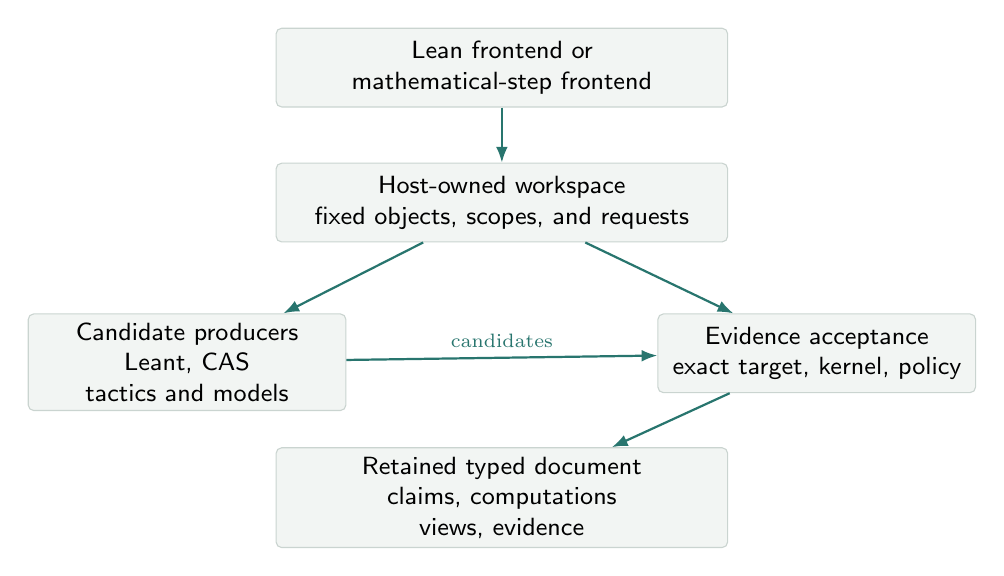
\begin{tikzpicture}[
 box/.style={draw=rulegray,fill=paperpanel,rounded corners=2pt,
   align=center,text width=5.5cm,minimum height=1cm,font=\small\sffamily},
 arr/.style={-{Latex[length=2mm]},thick,color=accent},node distance=7mm]
 \node[box] (input) {Lean frontend or mathematical-step frontend};
 \node[box,below=of input] (host) {Host-owned workspace\\fixed objects, scopes, and requests};
 \node[box,below left=9mm and -9mm of host,text width=3.8cm] (producer)
   {Candidate producers\\Leant, CAS\\tactics and models};
 \node[box,below right=9mm and -9mm of host,text width=3.8cm] (checker)
   {Evidence acceptance\\exact target, kernel, policy};
 \node[box,below=26mm of host] (artifact)
   {Retained typed document\\claims, computations\\views, evidence};
 \draw[arr] (input)--(host);
 \draw[arr] (host)--(producer);
 \draw[arr] (host)--(checker);
 \draw[arr] (producer)--node[above,font=\scriptsize]{candidates}(checker);
 \draw[arr] (checker)--(artifact);
\end{tikzpicture}
\end{center}

Producers may suggest objects and plans, but do not own the authoritative target supplied
to the checker. Operational isolation protects the checking environment from
executed metaprograms; ordinary typing alone does not provide that isolation.

\subsection{Freeze the meaning after resolving the statement's own constraints}
A statement seal records its elaborated expression, universe parameters,
ordered binders, selected structures and instances, relevant definitions,
and environment identity. It is created only when unresolved constraints that
could change the statement have been resolved or made explicit parameters.
Freezing should not be defined merely as assuming that a particular parser
callback always finishes the header independently of everything else.

Proof reconstruction cannot instantiate a remaining meaning-bearing hole to
select an easier theorem. When a statement genuinely needs clarification,
the source remains unresolved rather than being marked proved under the most
convenient interpretation. The same discipline applies to the input and result
specification of a CAS request.

The reader-facing statement view should disclose meaningful conventions:
truncated subtraction, total division, quantifier dependence, formal versus
analytic objects, selected branches, and local versus global hypotheses.
These are notices, not automatic accusations of an error. The author may
intend a total operator or a vacuous implication. An inconsistent local
context may legitimately appear in a proof by contradiction; the system
must not pretend to decide the consistency of arbitrary assumptions.

\subsection{Assembly and document coverage}
Each method instance has a checked combiner from its child obligations to its
claimed result. An unfinished proof can be represented by a typed term
$K:\Pi(h_1:Q_1)\cdots(h_m:Q_m),T$, with later obligations instantiated by earlier
accepted choices. Substituting correctly typed evidence produces a term of $T$.
This is ordinary dependent application, not a new soundness principle. The
assembled root term is then checked again at the fixed target.

The publication gate checks every asserted formal node, not just the final
root. Otherwise a false, unused intermediate sentence could coexist with a
valid theorem proof. A true but unused assertion may be retained as exposition
and marked unused. Free explanatory prose is not automatically a formal claim;
the document should visually distinguish it from the checked assertion layer.

Method-constrained nodes also retain the instantiated contract and its
obligations. Merely finding the method's name somewhere in a proof term is not
a conformance check. Conversely, conformance to the contract does not prove
that a reader will find the explanation illuminating.

\subsection{When may a data choice be automatic?}
The strongest general permission comes from uniqueness. If the specification
of an object has a proof
\[
 \forall a,b,\ \Spec(i,a)\to\Spec(i,b)\to a=b,
\]
then any two checked outputs denote the same object. A change of executable
representation can be justified through this equality and the relevant
transport theorem. The dyadic germ is exactly such an object.

Uniqueness does not imply that every representation has the same cost or
readability, and an explicit construction may still be of mathematical
interest. But it removes a semantic ambiguity that exists for an arbitrary
inhabitant of a weak type. Without uniqueness or another specified equivalence,
changing a retained data object is a visible edit. A proof-only replacement
of evidence for the same fixed proposition has a different status.

\subsection{A reproducible artifact has two useful representations}
The publication bundle should retain a readable source and an evidence form.
An expanded Lean file is the natural interoperability companion. A typed
certificate or exported proof-term form supports replay without rediscovering
the proof. The bundle also records source anchors, exact targets, selected
objects, view routes, dependencies, operational policy versions, and the
transitive axiom inventory.

Search-free replay does not mean computation-free replay. A reflected proof
may perform substantial deterministic reduction. Nor does a retained tactic
script automatically constitute search-free evidence: it may rerun
simplification, typeclass resolution, or theorem search. The syntheses' careful
distinction between frozen tactic text and retained terms should remain part
of the public contract~\cite{synthesis,blueprints}.

Replaying in a pinned environment and repairing for a new environment are
different operations. After a library upgrade, the old evidence still belongs
to the old environment. A repaired source or proof gets a new acceptance record,
with a semantic comparison of the statements and accepted objects. A failed
replay is not permission to strengthen the theorem until the new script works.

\subsection{Cache keys and semantic edits}
For a first implementation, key reuse by the complete immutable workspace
revision and exact request. This may invalidate more work than necessary,
but it is easy to reason about. Later, a dependency-aware cache can use the
closed semantic inputs actually needed by a node. Every reused item is still
checked against the current requested interface.

The cache must distinguish a changed definition or instance even when the
printed statement is unchanged. An explicit context embedding is needed to
reuse a local fact under renamed or extended binders. A branch-local result
cannot be retrieved simply because its printed target matches one outside
the branch.

The syntheses' edit classification is a useful default: evidence-only,
plan change, object change, and statement change~\cite{synthesis}. Add precision
or domain changes as semantic fields of the affected object or result relation.
Increasing a jet precision, dropping a domain restriction, or changing a
principal branch is not a harmless formatting edit.

\subsection{Method contracts should have stable project-facing names}
Use project-local theorem wrappers or aliases as the public method API where
upstream binder names are unstable. Attach roles to resolved binders and verify
the expected telescope when registering the method. Keep logical theorem
identity, operational discharge policy, and rendering template versions
separate. Inferring that every propositional binder is a routine side condition
would be a mistake: a theorem's principal mathematical hypothesis is often a
proposition too.

This is also the collaboration rule. A project owns its aliases and policies;
upstream library maintenance does not silently change which inputs an author
must supply. A migration can update those records, but it is tested and reviewed
like any other API migration.

\section{Performance and the first implementation}
\label{sec:implementation}

\subsection{Keep computation cheap enough to be usable}
The main risks are repeated elaboration, representation conversion, certificate
size, and kernel replay cost. A workspace can help only if it shares the relevant
objects without accidentally retaining every failed search state forever.
Use immutable semantic nodes and separately collectible exploration records.
An accepted object retains its evidence; a failed attempt may retain only a
bounded diagnostic summary.

Computational representations should use concrete finite data suitable for
evaluation. The general mathematical API can remain abstract or noncomputable,
provided a proved correspondence connects it to the executable data. This is
the same separation highlighted by the recent polynomial-tactics work in Lean
~\cite{polynomial-lean}; it is not solved by asking a general mathematical
polynomial type to serve every runtime purpose.

For evidence, prefer shared helper theorems and reflected certificates over
huge duplicated rewrite traces. Retain enough intermediate structure to explain
the argument, but do not expand a multiplication algorithm into thousands of
reader-visible equalities. Measure proof size and checking cost separately:
a compact-looking term can still demand expensive reduction.

The first scheduler should be deliberately simple. A bounded exact arithmetic
and local-theorem profile handles routine guards. Leant handles structural
requests only after that boundary is stable. General model-driven exploration
and conditional equality saturation are optional later providers, not reasons
to postpone a useful core.

\subsection{Proposed module boundaries}
\begin{tabularx}{\textwidth}{@{}P{.24\textwidth}Y@{}}
\toprule
Module & Responsibility\\
\midrule
\code{Locus.Core} & Typed nodes, ordered contexts, object identity, claim coverage,
statement and request seals.\\
\code{Locus.Method} & Annotated theorem contracts, structural plans, scoped
obligations, exact method-instance records.\\
\code{Locus.Compute} & Denotation interfaces, verified algorithms, certificate
checkers, result relations, precision contracts.\\
\code{Locus.Views} & Explicit representation routes, guards, transport, and
registered coherence evidence.\\
\code{Locus.Worker} & Isolated execution, request origins, budgets, cancellation,
transactional commits, exact candidate replay.\\
\code{Locus.Leant} & Structural abstraction, opaque-expression handles,
provider exchange, and candidate/evidence association.\\
\code{Locus.Document} & Lean and step frontends, source maps, mathematical
rendering, semantic differences, artifact export.\\
\bottomrule
\end{tabularx}
These names describe a proposed package split, not existing modules.
The trusted logical content remains ordinary Lean declarations and checked
terms. The operational implementation still needs testing and isolation;
calling its producers logically untrusted does not make all implementation
bugs irrelevant.

\subsection{A sequence of acceptance gates, not a funding roadmap}
\textbf{Gate A: one end-to-end mathematical computation.}
Implement exact rational polynomial arithmetic and the dyadic residual-to-jet
lemma in Lean. Accept an externally supplied finite jet and reject the wrong
branch and insufficient-precision neighbors. Expose the same checker through
ordinary Lean and a minimal \code{compute} node. Retain and replay the evidence
without rerunning coefficient discovery.

\textbf{Gate B: representation and local context.}
Implement domain-preserving cancellation and one explicit two-stage view route.
Add finite reindexing and the local-derivative contract as ordinary shared
lemmas. Show the missing endpoint and pointwise-only derivative failures at
the precise source nodes. Preserve the original group and local-analysis
generality of the ProveIt examples.

\textbf{Gate C: definitions and efficient verified production.}
Add a constructive coefficient producer, the theorem identifying it with the
specified root, and backward precision planning. Compare the triangular and
Newton producers at the same output relation. Add a competing third view and
check route stability rather than selecting one by whichever proof is easiest.

\textbf{Gate D: the Leant adapter.}
Connect structural requests with exact host-owned targets. Test exact displayed
edit replay, separate completion statuses, shared metavariables, stale results,
and cancellation. Data requests receive explicit specifications; finite behavioral
tests are not promoted to universal claims.

\textbf{Gate E: the frontend comparison.}
Lift a small set of existing Lean proofs into the shared document model and run
the comparative study below. Expand notation and method coverage only in
response to observed deficiencies. A polished standalone syntax is not required
to reach this gate.

\section{Evaluation that can reject the language hypothesis}
\label{sec:evaluation}

\subsection{Three treatments and separate sources of improvement}
Compare the original idiomatic Lean development, refactored Lean with the same
methods and certified-CAS packages, and the proposed workspace surface using
identical packages. The first difference measures total infrastructure benefit.
The second isolates the additional frontend and workspace interaction benefit.
If ordinary Lean already has the same persistent workspace services, compare
only the different authoring and reading forms at that stage.

Then ablate workspace representation sharing, automatic guard reuse, structured
method explanations, and new notation separately. A shorter proof obtained by
a new helper theorem is a library gain. A faster build obtained by reusing a
reified polynomial is a representation-sharing gain. A reader locating a wrong
branch more quickly may be a presentation gain. None should be credited to
surface syntax without the corresponding control.

The source audit in the syntheses can prioritize sampling, particularly local
analysis, but actual goals and outcomes must be instrumented. A tactic-head
classification cannot tell whether a premise was mathematically routine or
whether many failed attempts preceded the final short proof.

\subsection{A deliberately heterogeneous benchmark}
Use the three inspected ProveIt files as development examples, then hold out
related but nonidentical modules. The initial task families should include:
finite reindexing, local differentiation, a general-ring coefficient problem,
a newly defined formal root with computed jets, branch-sensitive algebraic
identification, and a certified numerical enclosure. Include already-short
wrappers as negative controls for unnecessary verbosity.

Split by theorem or module before harvesting subgoals. Exclude the target
and its downstream consequences from retrieval, including aliases, generated
examples, imported answer packages, and caches. A provider that retrieves a
preexisting proof of the benchmark target has not demonstrated reconstruction
of the omitted argument. Keep a manifest of the allowed environment for each
run.

The negative suite is not simply a list of false statements. Some mutations
invalidate a particular method while leaving the theorem true. Others change
the requested meaning, precision, or branch. The expected outcome must say
which boundary failed and why. Appendix~\ref{app:tests} gives a concrete plan.

\subsection{Measure effort, comprehension, and cost separately}
Record time and editing actions to a completed proof, the number of substantive
choices requested from the author, failed attempts, and repair effort after
small changes. In a separate reader task, ask participants to explain the
central argument, locate a missing hypothesis, and predict the effect of a
changed domain or precision. Counterbalance task order and record prior Lean
and subject experience.

For the implementation, measure total elaboration work, repeated reifications,
peak memory, candidate-generation and checking cost, median and tail latency,
certificate size, replay cost, and cancellation behavior. Also charge the work
of writing and maintaining adapters, reflection theorems, and generated interface
lemmas. With shared-library cost $L$, per-example authoring cost $A_i$, and
repair cost $R_i$, report
\[
 L,\quad (A_i)_i,\quad(R_i)_i,\quad
 L+\sum_i(A_i+R_i),
\]
not just the final source line count. Amortization should use demonstrated reuse,
not an assumed infinite future corpus.

A change to an index bound, a base-point unit hypothesis, a branch, an instance,
a coefficient convention, or a precision demand should be included in the
maintenance study. The system must preserve the theorem's actual generality,
not compensate for a difficult repair by strengthening the statement.

\subsection{Stopping rules}
Exact-target preservation, correct treatment of the negative neighbors, and
complete assertion coverage are correctness gates. Numerical usability thresholds
should be chosen after a pilot supplies realistic variance, rather than invented
here. Publish failed tasks and the required new library work alongside successes.

If the CAS packages and workspace API help but the new source language does
not improve authoring or reading, keep the packages and ship the document view
as an optional layer over Lean. If the surface improves reading but makes
authoring slower, a generated exposition may be the right product. Those are
useful outcomes, not failures to defend a predetermined language design.

\section{The executed companion and the remaining work}
\label{sec:demo}

\subsection{What was run}
The archive includes \code{certificate_demo.py}, a Python 3.9-or-later program
using only the standard library. All arithmetic uses integers and
\code{fractions.Fraction}. Its producer and checker paths are deliberately
separate: the jet producer uses the recurrence, while the checker evaluates
the residual; the bracket producer bisects, while the checker tests endpoint
signs; the radical checker combines exact algebra with independently checked
rational bounds.

The recorded execution passed \textbf{24 test methods}, with zero failures or
errors. Parameterized cases include jets at precisions $1$ through $24$,
coefficient-formula checks through degree $24$, and \textbf{702} finite binomial
orthogonality instances. Other tests cover endpoint omissions, the wrong
quadratic branch, corrupted coefficients, invalid radical bounds, wrong
principal-root signs, precision loss under differentiation, totalized division,
and nonunits modulo $6$. The machine-readable \code{test-results.json} retains
the actual interpreter version and the computed rational data.

These tests establish that the supplied arithmetic demonstrator executes as
reported. They do not formally verify its Python implementation, prove the
universal binomial identity by testing, or validate a Lean frontend. The
universal arguments are written in the article; translating the computational
contracts and those arguments into Lean is Gate A, not a completed result.

\subsection{The unresolved technical questions are now narrower}
The largest implementation questions are the cost of kernel-checkable reflection,
how much representation reuse survives realistic dependent contexts, how to
expose guards without overwhelming readers, and which definitions benefit from
an executable refinement interface. Each now has a concrete experiment rather
than only a general aspiration.

More ambitious extensions remain plausible: automatic discovery of reusable
computational theories, certified asymptotic manipulation, learning method
selection from completed workspaces, and transporting results between equivalent
mathematical presentations. They should preserve the same boundary: generated
plans may be speculative; their accepted mathematical outputs must have exact,
scoped, checked specifications.

\subsection{Conclusion}
The first round identified the right conservative foundation. The next step
should be more ambitious about mathematical objects and computation, not about
replacing the kernel or multiplying proof keywords.

\Locus{} makes a proof assistant and a verified CAS parts of one mathematical
workspace. A theorem application produces evidence, a computation produces an
object together with a relation, a view changes representation through a theorem,
and a precision annotation states an exact observation rather than an informal
promise. Leant contributes structural discovery without becoming the authority
for the statement. The human author retains the argument's choices, while
shared context and verified algorithms reconstruct their formal consequences.

The formal-root example is the proposed first implementation target because it
exercises the whole idea in a bounded setting: definition, uniqueness, executable
representation, symbolic computation, branch selection, precision, and compact
certificate checking. Building that path in Lean, and making it equally usable
from ordinary Lean, would advance the brainstorm more than another broad
manifesto about human-like proof syntax.

\appendix
\section{Minimal semantic interfaces}
\label{app:interfaces}

These interfaces are design-level descriptions. They are not claimed to be
compilable Lean source.

\subsection{An operation record}
\begin{lstlisting}
Operation {
  node_id,
  origin,
  exact_input_telescope,
  input_objects,
  output_family,
  requested_relation,
  semantic_mode,         // exact, local, partial, jet, enclosure, ...
  method_or_theory_id,
  selected_view_route,
  generated_obligations,
  accepted_output,       // absent until a candidate is selected
  proof_of_relation,     // absent until checked
  source_map,
  dependency_inventory
}
\end{lstlisting}
The semantic mode is a readable classifier; the actual authority is the resolved
relation. A forged \code{Exact} tag cannot turn a proof of a jet congruence into
a proof of equality. Likewise, a requested domain is represented inside the
relation, not only in a UI field.

\subsection{The positive acceptance rule}
With all entries interpreted in the same validated context,
\[
 \frac{\Gamma\vdash i:I\qquad
       \Gamma\vdash o:O(i)\qquad
       \Gamma\vdash p:\Spec(i,o)}
      {\Gamma\vdash\operatorname{accept}(i,o,p):
         \{o:O(i)\mid\Spec(i,o)\}}.
\]
This rule describes the logical payload. Publication additionally checks exact
request identity, permitted dependencies, all source assertions, and the
selected method-conformance policy. These operational checks should not be
mistaken for additional logical axioms.

For a conditional output with a guard $G(i,o)$, the proof has type
$G(i,o)\to\Spec(i,o)$ until the guard is discharged. The UI may preview the
candidate but cannot present $\Spec(i,o)$ as proved unconditionally. For a
refinement, the checked output is a combiner from the exact child obligations;
it is not evidence that those children are already solved.

\Needspace{22\baselineskip}
\subsection{A computational theory registration}
\begin{lstlisting}
ComputationalTheory {
  semantic_domain,
  syntax_and_variable_model,
  denotation,
  reification_correspondence,
  supported_operation_contracts,
  verified_algorithms,
  certificate_formats_and_sound_checkers,
  guard_derivation_rules,
  precision_transfer_theorems,
  presentation_and_cost_policy,
  negative_neighbor_suite
}
\end{lstlisting}
An implementation may split these fields across ordinary Lean modules. The
logical components are definitions and theorems. Operational policy, resource
limits, and formatting are versioned separately. A package registration can
check that the required declarations have the expected types; it need not
introduce a new trusted contract interpreter.

\section{Proposed integration test matrix}
\label{app:tests}

This is a specification for a future Lean implementation. The Python companion
exercises selected arithmetic premises and counterexamples, not this whole
integration matrix.

\small
\begin{longtable}{@{}P{.06\textwidth}P{.41\textwidth}P{.45\textwidth}@{}}
\toprule
ID & Mutation & Required behavior\\
\midrule
\endhead
T01 & Remove the upper endpoint from binomial reindexing. & The method fails on
surjectivity or coverage of the inclusive endpoint; an unrelated proof does
not validate the reindexing plan.\\
T02 & Use a noninjective map for an unweighted finite reindexing. & Demand a
bijection or a different multiplicity-aware theorem.\\
T03 & Apply the finite-sum method to an infinite series. & Require the applicable
summability and rearrangement contract.\\
T04 & Replace neighborhood equality by equality at one point. & Local derivative
transfer remains open, naming the missing eventual equality.\\
T05 & Supply only pointwise convergence for a limit interchange. & The chosen
analytic theorem's additional hypotheses remain explicit.\\
T06 & Replace a unit coefficient by a merely nonzero coefficient over a ring. &
Reject the unit-based inversion method without strengthening the ring.\\
T07 & Remove a cancellation domain restriction. & Do not promote equality on
$x\neq1$ to global equality of total real expressions.\\
T08 & Normalize a partial function and then forget its domain. & Keep the original
domain; a wider extension must be a new specified object.\\
T09 & Return the negative denesting candidate with the correct square. & Reject
the principal-root specification at the sign or branch obligation.\\
T10 & Return the quadratic formal root with constant $-1/4$. & Reject the
zero-constant root request even if its residual vanishes.\\
T11 & Request precision $N+1$ from a certificate modulo $Q^N$. & Keep the higher
precision obligation open or recompute and verify additional coefficients.\\
T12 & Differentiate a jet while retaining its old precision. & Lower the output
precision or request one more input order.\\
T13 & Evaluate a formal jet as an analytic error bound. & Require a realization
and remainder theorem, not merely a formal congruence.\\
T14 & Present one root as a complete solution list. & Demand the quantified
completeness theorem, separately from membership of the root.\\
T15 & Reuse a branch-local fact outside its scope. & Reject the missing context
embedding, including when the result comes from a cache.\\
T16 & Change an instance while leaving printed notation unchanged. & Invalidate
or recheck the semantic interface and show the changed operations.\\
T17 & Let proof search instantiate a meaning-bearing statement hole. & Keep the
statement unresolved or request a visible source change.\\
T18 & Have a probe print a different, invalid suggested replacement. & Reject the
exact displayed edit even when the probe itself succeeded.\\
T19 & Receive a valid late result after undo. & Do not commit it to a different
origin; retain it only as an obsolete result.\\
T20 & Close one goal while other goals remain. & Report local completion, not
whole-proof completion or publication readiness.\\
T21 & Include an unapproved axiom in a transitive dependency. & Fail the publication
policy even if the root term is accepted relative to that axiom.\\
T22 & State a false but unused formal checkpoint. & Reject document coverage even
when the final theorem has another valid proof.\\
T23 & Add a constructor to a datatype handled by a structural plan. & Recompute
coverage; do not reuse a stale list of handled constructors.\\
T24 & Exhaust structural or CAS search. & Return budget/fragment information,
never an invented mathematical negation.\\
T25 & Supply a finite behavioral test for a universal specification. & Retain the
finite fact and leave the universal obligation unsolved.\\
T26 & Introduce a second meaning-bearing representation route. & Preserve the
selected route, request a choice, or apply a checked coherence theorem.\\
T27 & Retrieve the benchmark's own target through an alias. & Mark the benchmark
run invalid under the declared dependency-exclusion policy.\\
T28 & Solve sibling obligations with incompatible shared data assignments. &
Reject an inconsistent commit and restore the unchanged origin.\\
\bottomrule
\end{longtable}
\normalsize

\section{Source register and reading map}
\label{app:sources}

The source identifiers below are \emph{Git blob SHAs}, not repository commit
SHAs. They identify the file contents returned by the GitHub connector during
this review. Branch URLs in the bibliography are convenient navigation links;
the blob identifiers preserve which contents were inspected if those branches
subsequently move. The machine-readable \code{source-register.json} contains
the full paths, URLs, identities, and scope notes. The archive does not include
copies of the repositories.


\Needspace{4\baselineskip}\textbf{Brainstorm: primary synthesis.}\par
\code{docs/synthesis/unified-report.tex}\\
Blob \code{4bfcf344c91562fd7926a46a89bd78307b1ea750}. Read for consensus,
method and obligation semantics, Leant review, revisions concerning the second
report, and the next-round experimental questions~\cite{synthesis}.

\Needspace{4\baselineskip}\textbf{Brainstorm: comparative report.}\par
\code{docs/unified_report/unified_report.tex}\\
Blob \code{e99c39f64a67eaad8e3dc487104951a522494f6a}. Read for the feature
comparison, reported lexical audit, annotated-theorem interface, definitions
question, updated qualifications, and detailed Leant discussion~\cite{blueprints}.

\Needspace{4\baselineskip}\textbf{ProveIt: binomial inversion.}\par
\code{Analysis/FabiusFunction/Lean/FabiusFunction/BinomialInversion.lean}\\
Blob \code{c6b0fe63a4faf8708b71e9b93aa2ce7406464d84}. Direct full-file static
reading; emphasis on kernel orthogonality, index/cast bridges, and preservation
of additive-group generality~\cite{p-binomial}.

\Needspace{4\baselineskip}\textbf{ProveIt: autonomous derivatives.}\par
\code{Analysis/FabiusFunction/Lean/FabiusFunction/AutonomousIteratedDeriv.lean}\\
Blob \code{1422b87f31073fed898ff0c8a080ea0a798aef5e}. Direct full-file static
reading; emphasis on the range-local hypotheses and the neighborhood equality
used in the induction step~\cite{p-ode}.

\Needspace{4\baselineskip}\textbf{ProveIt: algebraic germ.}\par
\code{Analysis/FabiusFunction/Lean/FabiusFunction/AlgebraicInverseGerm.lean}\\
Blob \code{b7bd59bf3f940f965e1936942d0ea6adfb4e03d6}. Direct full-file static
reading; emphasis on coefficient transport, unit-based unique roots, and the
concrete quadratic dyadic instance~\cite{p-germ}.

\Needspace{4\baselineskip}\textbf{Leant: verification boundary.}\par
\code{src/Leant/Synth/Verification.hs}\\
Blob \code{caee3c51cfd226e6c2bb9887f80293343abd486c}. Direct full-file static
reading of callback receipts, candidate variants, quotas, and accepted-spelling
deduplication~\cite{l-verify}.

\Needspace{4\baselineskip}\textbf{Leant: engine boundary.}\par
\code{src/Leant/Synth/Engine.hs}\\
Blob \code{1064c8215506e172401cd7c5c06d7e8222e0befa}. Direct reading of the
module header and interface (lines 1--180), not an audit of the entire engine
implementation~\cite{leant-engine}.

\Needspace{4\baselineskip}\textbf{Leant: synthesis internals.}\par
\code{docs/synth-internals.md}\\
Blob \code{1723e1409060ee9eaabe21ae2ca9c37be6eaa9a7}. Direct reading of the
opening implementation and provenance discussion (lines 1--190), including the
distinction between historical and newer acceptance receipts~\cite{l-internals}.


Repository test counts appearing in those sources remain attributed historical
or documented results. The only new execution receipt in this archive is the
Python companion's \code{test-results.json}. No inference of whole-corpus proof
completeness is made from a textual absence of \code{sorry}.

\clearpage
\phantomsection
\addcontentsline{toc}{section}{References}
\begin{thebibliography}{99}
\small

\bibitem{synthesis}
Brainstorm contributors.
\emph{Mathematical Ideas, Checked Evidence: A Unified Evaluation of Nine
Proof-Language Proposals}. Revised synthesis, 5 September 2026.
\url{https://github.com/VladimirReshetnikov/Brainstorm/blob/main/docs/synthesis/unified-report.tex}.
File identity recorded in Appendix~\ref{app:sources}.

\bibitem{blueprints}
Brainstorm contributors.
\emph{Nine Blueprints for a Mathematician's Proof Language over Lean}.
Revised comparative report, 5 September 2026.
\url{https://github.com/VladimirReshetnikov/Brainstorm/blob/main/docs/unified_report/unified_report.tex}.
File identity recorded in Appendix~\ref{app:sources}.

\bibitem{p-binomial}
Vladimir Reshetnikov and contributors.
\emph{ProveIt: BinomialInversion.lean}.
\url{https://github.com/VladimirReshetnikov/ProveIt/blob/main/Analysis/FabiusFunction/Lean/FabiusFunction/BinomialInversion.lean}.
Inspected 5 September 2026.

\bibitem{p-ode}
Vladimir Reshetnikov and contributors.
\emph{ProveIt: AutonomousIteratedDeriv.lean}.
\url{https://github.com/VladimirReshetnikov/ProveIt/blob/main/Analysis/FabiusFunction/Lean/FabiusFunction/AutonomousIteratedDeriv.lean}.
Inspected 5 September 2026.

\bibitem{p-germ}
Vladimir Reshetnikov and contributors.
\emph{ProveIt: AlgebraicInverseGerm.lean}.
\url{https://github.com/VladimirReshetnikov/ProveIt/blob/main/Analysis/FabiusFunction/Lean/FabiusFunction/AlgebraicInverseGerm.lean}.
Inspected 5 September 2026.

\bibitem{l-verify}
Vladimir Reshetnikov and contributors.
\emph{Leant: Leant.Synth.Verification}.
\url{https://github.com/VladimirReshetnikov/Leant/blob/main/src/Leant/Synth/Verification.hs}.
Inspected 5 September 2026.

\bibitem{leant-engine}
Vladimir Reshetnikov and contributors.
\emph{Leant: Leant.Synth.Engine}, module boundary and exported interface.
\url{https://github.com/VladimirReshetnikov/Leant/blob/main/src/Leant/Synth/Engine.hs}.
Inspected 5 September 2026.

\bibitem{l-internals}
Vladimir Reshetnikov and contributors.
\emph{Leant: :synth internals}, opening provenance and implementation discussion.
\url{https://github.com/VladimirReshetnikov/Leant/blob/main/docs/synth-internals.md}.
Inspected 5 September 2026.

\bibitem{lean-validation}
The Lean development team.
\emph{Validating a Lean Proof}. Lean Language Reference.
\url{https://lean-lang.org/doc/reference/latest/ValidatingProofs/}.
Consulted 5 September 2026; native-computation policy is version-sensitive.

\bibitem{li-paulson}
Wenda Li, Grant Olney Passmore, and Lawrence C. Paulson.
\emph{Deciding Univariate Polynomial Problems Using Untrusted Certificates
in Isabelle/HOL}. Journal of Automated Reasoning, 2017;
arXiv:1506.08238v2, revised 10 April 2018.
\url{https://arxiv.org/abs/1506.08238v2}.
\url{https://doi.org/10.1007/s10817-017-9424-6}.

\bibitem{polynomial-lean}
Hao Shen, Junyu Guo, Junqi Liu, and Lihong Zhi.
\emph{Automated Tactics for Polynomial Reasoning in Lean 4}.
arXiv:2604.13514v1, 15 April 2026.
\url{https://arxiv.org/abs/2604.13514}.

\bibitem{verbose}
Patrick Massot.
\emph{Teaching Mathematics Using Lean and Controlled Natural Language}.
In ITP 2024, LIPIcs 309, pp.~27:1--27:19.
\url{https://doi.org/10.4230/LIPIcs.ITP.2024.27}.

\bibitem{isar}
The Isabelle project.
\emph{Isar: Intelligible semi-automated reasoning}.
\url{https://isabelle.in.tum.de/Isar/}.
Consulted 5 September 2026.

\end{thebibliography}
\end{document}
